\documentclass[10pt,a4paper]{article}
\usepackage[utf8]{inputenc}
\usepackage[T1]{fontenc}
%\usepackage{stringenc} % for grffile
%\usepackage{ucs}
\usepackage{amsthm} %numéroter les questions
\usepackage[english]{babel}
\usepackage{datetime}
\usepackage{scrextend} %\footref{}
\usepackage[normalem]{ulem}
\usepackage{xspace} % typographie IN
\usepackage{hyperref}% hyperliens
\usepackage[all]{hypcap} %lien pointe en haut des figures
\usepackage[english]{varioref} %voir x p y
\usepackage{fancyhdr}% en têtes
%\input cyracc.def
\usepackage[]{graphicx} %include pictures
%\usepackage[encoding,inputencoding=utf8,filenameencoding=utf8]{grffile}
%\usepackage[extendedchars,inputencoding=latin1,filenameencoding=latin1]{grffile}
\usepackage[siunitx ]{circuitikz}
%\usepackage{gnuplottex}
\usepackage{ifthen}
\graphicspath{{./figures/}}
%\usepackage{array}
\usepackage{amsmath}
\usepackage[]{xcolor}
\usepackage{tikz}
\usepackage{tikz-timing}
\usetikzlibrary{scopes}
\usetikzlibrary{backgrounds}
\usepackage{listings}
\usepackage{enumitem}
\usepackage[top=1 in, bottom=1 in, left=1.3 in, right=1 in]{geometry} % Yeah, that's bad to play with margins
\usepackage[]{pdfpages}
\usepackage{pdflscape}
\usepackage[]{attachfile}
%\usepackage{colortbl}
%\usepackage{multirow}
\usepackage{booktabs}
\usepackage{makecell}
\usepackage[ ]{subfig}
%\usepackage{rotating}

\newcommand{\version}{v1.0.0}

%cyr
%\newcommand\textcyr[1]{{\fontencoding{OT2}\fontfamily{wncyr}\selectfont #1}}


\newboolean{corrige}
%\setboolean{corrige}{true}%corrigé
\setboolean{corrige}{false}% pas de corrigé

\newboolean{annexes}
%\setboolean{annexes}{true}%annexes
\setboolean{annexes}{false}% pas de annexes

\newboolean{mos}
%\setboolean{mos}{true}%annexes
\setboolean{mos}{false}% pas de annexes

\usepackage{aeguill} %guillemets

%% fancy header & foot
\pagestyle{fancy}
\lhead{[ELEC-H-473] Microprocessor Architectures: RiSC16}
\rhead{\version\\ page \thepage}
\chead{\ifthenelse{\boolean{corrige}}{Corrigé}{}}
\cfoot{}
%%
%\fancypagestyle{plain}

\pdfinfo{
/Author (Yannick Allard, ULB -- BEAMS)
/Title (Lab 3 ELEC-H-473, RiSC16)
/ModDate (D:\pdfdate)
}

\hypersetup{
pdftitle={Lab 3 [ELEC-H-473] Microprocessor Architectures},
pdfauthor={Yannick Allard, 2013-2017 ULB - BEAMS  },
pdfsubject={RiSC16}
}

\theoremstyle{definition}% questions pas en italique
\newtheorem{Q}{Question}[] % numéroter les questions [section] ou non []

\newcommand{\reponse}[1]{% pour intégrer une réponse : \reponse{texte} : sera inclus si \boolean{corrige}
	\ifthenelse {\boolean{corrige}} {\paragraph{Réponse :} #1} {}
 }

\newcommand{\addcontentslinenono}[4]{\addtocontents{#1}{\protect\contentsline{#2}{#3}{#4}{}}}

\newcommand{\on}[1]{\operatorname{#1}}

\newcommand{\reg}[1]{\texttt{reg#1}}

\def\labelitemi{--}
\setlist{parsep=0pt,itemsep=0pt,style=standard,leftmargin=\parindent, align=left} % pas d'espace prohibitif entre les items
\setlist{nolistsep}

\newcolumntype{C}[1]{>{\centering\let\newline\\\arraybackslash\hspace{0pt}}m{#1}}

%\setlength{\tabcolsep}{0pt} %no extra space in cells to keep constant tabular width

\date{\vspace{-1cm}\version}
\title{\vspace{-2cm} Lab 3\\ Microprocessor Architectures [ELEC-H-473]\\ RiSC16: internal processor behaviour  \ifthenelse{\boolean{corrige}}{~\\Corrigé}{}}

%\author{\vspace{-1cm}}%\textsc{Yannick Allard}}


\lstdefinestyle{customasm}{
 % belowcaptionskip=1\baselineskip,
 % frame=L,
 % xleftmargin=\parindent,
  language=[x86masm]Assembler,
  basicstyle=\footnotesize\ttfamily,
  commentstyle=\itshape\color{purple!40!black},
  comment=[l]//,
}

\lstset{escapechar=@,style=customasm}

\begin{document}

% Introduce a new counter for counting the nodes needed for circling
\newcounter{nodecount}
% Command for making a new node and naming it according to the nodecount counter
\newcommand\tabnode[1]{\addtocounter{nodecount}{1} \tikz \node (\arabic{nodecount}) {#1};}

% Some options common to all the nodes and paths
\tikzstyle{every picture}+=[remember picture,baseline]
\tikzstyle{every node}+=[inner sep=0pt,anchor=base]
\tikzstyle{every path}+=[thick, rounded corners]

% for tikz pict


\maketitle
\section*{Introduction}
%\section{Introducvtion}

This lab about the RiSC16 will highlight the limitations of the RiSC16's 8-instruction architecture. The simulator you will use in this lab will enable you to define a new architecture with additional instructions and additional registers.

%Ce dernier labo mettra en évidence les limites du jeu d'instruction réduit du RiSC16.
%Le simulateur que vous utiliserez vous permettra de définir une autre architecture possédant de nouvelles instructions et un nombre différent de registres.

Processor performances can be characterised by the time ($t$) required to execute a program and depends on:
\begin{itemize}
\item the number of instructions executed $\on{CI}$
\item the average number of cycles per instruction $\on{CPI}$
\item the clock frequency $f$
\end{itemize}

Thus the equation is:
%$$t=1/\on{performance}$$
%
\begin{eqnarray*}
t & = & \frac{1}{\on{performance}}\\
& = & (\on{instruction~ number})\cdot(\on{cycles~ per~ instruction})\cdot(\on{clock~ period})\\
& = & \frac{\on{CI}\cdot \on{CPI}}{f} \\
\end{eqnarray*}

%On peut caractériser la performance d'un processeur par le temps qu'il faut pour exécuter un programme. Le temps d'exécution dépend de trois facteurs :
%le nombre d'instructions machine exécutées (IC) ;
%le nombre moyen de cycles par instruction (CPI) ;
%la fréquence de l'horloge (f).
%Mis en équation, on a :

%	temps 	= 1/ performance
%		= (nombre d’instructions) x (nombre de cycles par instruction) x	(période d’horloge)

The possibilities to improve performance are to:
\begin{itemize}
\item increase clock frequency ($f$)
\item change processor internal design to lower $\on{CPI}$
\item optimise the compiler to reduce the number of instructions ($\on{CI}$) or decrease $\on{CPI}$
\item extend the instruction set to decrease $\on{CI}$
\end{itemize}



%Il est donc possible d'améliorer les performances par les moyens suivants :
%augmenter la fréquence d'horloge (f).
%augmenter l'organisation interne pour diminuer le CPI.
%optimiser le compilateur pour diminuer le nombre d'instructions exécutées (IC) ou le CPI.
%enrichir le jeu d'instructions pour qu'il y ait moins d'instructions à exécuter (IC).

In this lab, we will explore the last possibility and thus will extend the RiSC16 instruction set to 16 instructions.

%Lors de cette manipulation, nous allons nous intéresser plus précisément à ce dernier point.

\section{New instructions}

%Nouvelles instructions disponibles :

The 8-instruction set will be extended with 8 new instructions. As there are now 16 instructions, 4 bits must be used to code the opcode instead of 3. Instructions must be coded on 17 bits. This instruction set is detailed in Table \vref{tab:IS1}.

%\setlength{\tabcolsep}{5pt} %no extra space in cells to keep constant tabular width
%\setlength{\cmidrulewidth}{1pt}
\begin{table}[ht!]
	\begin{center}
%		\begin{tabular}{r|*{4}{c}|*{3}{c}|*{3}{c}|*{4}{c}|*{3}{c}}%m{1.2cm}m{8cm}}
%		\toprule
%		Instr/bit	& \multicolumn{4}{c|}{16--13}  & \multicolumn{3}{c|}{12--10}  & \multicolumn{3}{c|}{9--7}  & \multicolumn{4}{c|}{6--3}  & \multicolumn{3}{c}{2--0}\\
%		\midrule
%		ADD & \multicolumn{4}{c|}{0000} & \multicolumn{3}{c|}{reg A} & \multicolumn{3}{c|}{reg B} & \multicolumn{4}{c|}{(-8 to 7)} & \multicolumn{3}{c}{reg C} \\
%		SUB & \multicolumn{4}{c|}{0001} & \multicolumn{3}{c|}{reg A} & \multicolumn{3}{c|}{reg B} & \multicolumn{4}{c|}{(-8 to 7)} & \multicolumn{3}{c}{reg C} \\
%		NAND &\multicolumn{4}{c|}{0010} & \multicolumn{3}{c|}{reg A} & \multicolumn{3}{c|}{reg B} & \multicolumn{4}{c|}{0000} & \multicolumn{3}{c}{reg C} \\ \cmidrule{18-28} %\midrule
%		LUI & \multicolumn{4}{c|}{0011} & \multicolumn{3}{c|}{reg A} & \multicolumn{10}{c}{immediate 0 to 0x3FF} \\ %\cline{1-7}%\cmidrule(r){3-7}
%		\cmidrule{10-18}
%		SHL & \multicolumn{4}{c|}{0100} & \multicolumn{3}{c|}{reg A} & \multicolumn{3}{c|}{reg B} & \multicolumn{4}{c|}{(-8 to 7)} & \multicolumn{3}{c}{reg C} \\
%		SHA & \multicolumn{4}{c|}{0101} & \multicolumn{3}{c|}{reg A} & \multicolumn{3}{c|}{reg B} & \multicolumn{4}{c|}{(-8 to 7)} & \multicolumn{3}{c}{reg C} \\
%		NOR & \multicolumn{4}{c|}{0110} & \multicolumn{3}{c|}{reg A} & \multicolumn{3}{c|}{reg B} & \multicolumn{4}{c|}{0000} & \multicolumn{3}{c}{reg C} \\
%		\midrule
%		ADDI & \multicolumn{4}{c|}{1000} & \multicolumn{3}{c|}{reg A} & \multicolumn{3}{c|}{reg B} & \multicolumn{7}{c}{signed immediate (-64 to 63)} \\
%		SHIFTI & \multicolumn{4}{c|}{1001} & \multicolumn{3}{c|}{reg A} & \multicolumn{3}{c|}{reg B} & \multicolumn{7}{c}{signed immediate (-64 to 63)} \\
%		BL & \multicolumn{4}{c|}{1010} & \multicolumn{3}{c|}{reg A} & \multicolumn{3}{c|}{reg B} & \multicolumn{7}{c}{signed immediate (-64 to 63)} \\
%		BG & \multicolumn{4}{c|}{1011} & \multicolumn{3}{c|}{reg A} & \multicolumn{3}{c|}{reg B} & \multicolumn{7}{c}{signed immediate (-64 to 63)} \\
%		LW& \multicolumn{4}{c|}{1100} & \multicolumn{3}{c|}{reg A} & \multicolumn{3}{c|}{reg B} & \multicolumn{7}{c}{signed immediate (-64 to 63)} \\
%		SW& \multicolumn{4}{c|}{1101} & \multicolumn{3}{c|}{reg A} & \multicolumn{3}{c|}{reg B} & \multicolumn{7}{c}{signed immediate (-64 to 63)} \\
%		BEQ & \multicolumn{4}{c|}{1110} & \multicolumn{3}{c|}{reg A} & \multicolumn{3}{c|}{reg B} & \multicolumn{7}{c}{signed immediate (-64 to 63)} \\
%		JALR & \multicolumn{4}{c|}{1111} & \multicolumn{3}{c|}{reg A} & \multicolumn{3}{c|}{reg B} & \multicolumn{7}{c}{signed immediate (-64 to 63)} \\
%		\bottomrule
%		\end{tabular}
		\begin{tabular}{r|c|c|c|c|c}%m{1.2cm}m{8cm}}
		\toprule
		\diaghead{bourage~}{Instr}{ bit}	& 16--13  & 12--10  & {9--7}  & 6--3  & {2--0}\\
		\midrule
		ADD & 0000 & reg A & reg B & (-8 to 7) & {reg C} \\
		SUB & 0001 & reg A & reg B & (-8 to 7) & {reg C} \\
		NAND & 0010 & reg A & reg B & 0000 & {reg C} \\ \cmidrule{4-6} %\midrule
		LUI & 0011 & reg A & \multicolumn{3}{c}{immediate 0 to 0x3FF} \\ %\cline{1-7}%\cmidrule(r){3-7}
		\cmidrule{4-6}
		SHL & 0100 & reg A & reg B & (-8 to 7) & {reg C} \\
		SHA & 0101 & reg A & reg B & (-8 to 7) & {reg C} \\
		NOR & 0110 & reg A & reg B & 0000 & {reg C} \\
		XOR & 0111 & reg A & reg B & 0000 & {reg C} \\
		\cmidrule{5-6}
		ADDI & 1000 & reg A & reg B & \multicolumn{2}{c}{signed immediate (-64 to 63)} \\
		SHIFTI & 1001 & reg A & reg B & \multicolumn{2}{c}{signed immediate (-64 to 63)} \\
		BL & 1010 & reg A & reg B & \multicolumn{2}{c}{signed immediate (-64 to 63)} \\
		BG & 1011 & reg A & reg B & \multicolumn{2}{c}{signed immediate (-64 to 63)} \\
		LW& 1100 & reg A & reg B & \multicolumn{2}{c}{signed immediate (-64 to 63)} \\
		SW& 1101 & reg A & reg B & \multicolumn{2}{c}{signed immediate (-64 to 63)} \\
		BEQ & 1110 & reg A & reg B & \multicolumn{2}{c}{signed immediate (-64 to 63)} \\
		JALR & 1111 & reg A & reg B & \multicolumn{2}{c}{signed immediate (-64 to 63)} \\
		\bottomrule
		\end{tabular}
	\end{center}
\caption{Special IS[1]}
\label{tab:IS1}
\end{table}

%Le jeu d'instructions du RiSC16 complété par 8 nouvelles instructions est représenté sur le tableau ci-dessous (Special IS[1]). Puisque ce jeu d'instructions comporte 16 instructions, il faut 4 bits pour coder une instruction au lieu de 3. La taille d'une instruction passe donc de 16 bits à 17 bits.

The number of registers and the number of bits used for immediate constants can be adapted to make several flavours of the same processor. A variant using 24-bit instructions is defined in the simulator as in the Table \vref{tab:IS1-16-24}.

\begin{table}[ht!]
	\begin{center}
%		\begin{tabular}{r|*{4}{c}|*{3}{c}|*{3}{c}|*{4}{c}|*{3}{c}}%m{1.2cm}m{8cm}}
%		\toprule
%		Instr/bit	& \multicolumn{4}{c|}{16--13}  & \multicolumn{3}{c|}{12--10}  & \multicolumn{3}{c|}{9--7}  & \multicolumn{4}{c|}{6--3}  & \multicolumn{3}{c}{2--0}\\
%		\midrule
%		ADD & \multicolumn{4}{c|}{0000} & \multicolumn{3}{c|}{reg A} & \multicolumn{3}{c|}{reg B} & \multicolumn{4}{c|}{(-8 to 7)} & \multicolumn{3}{c}{reg C} \\
%		SUB & \multicolumn{4}{c|}{0001} & \multicolumn{3}{c|}{reg A} & \multicolumn{3}{c|}{reg B} & \multicolumn{4}{c|}{(-8 to 7)} & \multicolumn{3}{c}{reg C} \\
%		NAND &\multicolumn{4}{c|}{0010} & \multicolumn{3}{c|}{reg A} & \multicolumn{3}{c|}{reg B} & \multicolumn{4}{c|}{0000} & \multicolumn{3}{c}{reg C} \\ \cmidrule{18-28} %\midrule
%		LUI & \multicolumn{4}{c|}{0011} & \multicolumn{3}{c|}{reg A} & \multicolumn{10}{c}{immediate 0 to 0x3FF} \\ %\cline{1-7}%\cmidrule(r){3-7}
%		\cmidrule{10-18}
%		SHL & \multicolumn{4}{c|}{0100} & \multicolumn{3}{c|}{reg A} & \multicolumn{3}{c|}{reg B} & \multicolumn{4}{c|}{(-8 to 7)} & \multicolumn{3}{c}{reg C} \\
%		SHA & \multicolumn{4}{c|}{0101} & \multicolumn{3}{c|}{reg A} & \multicolumn{3}{c|}{reg B} & \multicolumn{4}{c|}{(-8 to 7)} & \multicolumn{3}{c}{reg C} \\
%		NOR & \multicolumn{4}{c|}{0110} & \multicolumn{3}{c|}{reg A} & \multicolumn{3}{c|}{reg B} & \multicolumn{4}{c|}{0000} & \multicolumn{3}{c}{reg C} \\
%		\midrule
%		ADDI & \multicolumn{4}{c|}{1000} & \multicolumn{3}{c|}{reg A} & \multicolumn{3}{c|}{reg B} & \multicolumn{7}{c}{signed immediate (-64 to 63)} \\
%		SHIFTI & \multicolumn{4}{c|}{1001} & \multicolumn{3}{c|}{reg A} & \multicolumn{3}{c|}{reg B} & \multicolumn{7}{c}{signed immediate (-64 to 63)} \\
%		BL & \multicolumn{4}{c|}{1010} & \multicolumn{3}{c|}{reg A} & \multicolumn{3}{c|}{reg B} & \multicolumn{7}{c}{signed immediate (-64 to 63)} \\
%		BG & \multicolumn{4}{c|}{1011} & \multicolumn{3}{c|}{reg A} & \multicolumn{3}{c|}{reg B} & \multicolumn{7}{c}{signed immediate (-64 to 63)} \\
%		LW& \multicolumn{4}{c|}{1100} & \multicolumn{3}{c|}{reg A} & \multicolumn{3}{c|}{reg B} & \multicolumn{7}{c}{signed immediate (-64 to 63)} \\
%		SW& \multicolumn{4}{c|}{1101} & \multicolumn{3}{c|}{reg A} & \multicolumn{3}{c|}{reg B} & \multicolumn{7}{c}{signed immediate (-64 to 63)} \\
%		BEQ & \multicolumn{4}{c|}{1110} & \multicolumn{3}{c|}{reg A} & \multicolumn{3}{c|}{reg B} & \multicolumn{7}{c}{signed immediate (-64 to 63)} \\
%		JALR & \multicolumn{4}{c|}{1111} & \multicolumn{3}{c|}{reg A} & \multicolumn{3}{c|}{reg B} & \multicolumn{7}{c}{signed immediate (-64 to 63)} \\
%		\bottomrule
%		\end{tabular}
		\begin{tabular}{r|c|c|c|c|c}%m{1.2cm}m{8cm}}
		\toprule
		\diaghead{bourage~}{Instr}{ bit}	& 23--20  & 19--16  & {15--12}  & 11--4  & {3--0}\\
		\midrule
		ADD & 0000 & reg A & reg B & (-128 to 127) & {reg C} \\
		SUB & 0001 & reg A & reg B & (-128 to 127) & {reg C} \\
		NAND & 0010 & reg A & reg B & 00000000 & {reg C} \\ \cmidrule{4-6} %\midrule
		LUI & 0011 & reg A & \multicolumn{3}{c}{immediate 0 to 0xFFFF} \\ %\cline{1-7}%\cmidrule(r){3-7}
		\cmidrule{4-6}
		SHL & 0100 & reg A & reg B & (-128 to 127) & {reg C} \\
		SHA & 0101 & reg A & reg B & (-128 to 127) & {reg C} \\
		NOR & 0110 & reg A & reg B & 00000000 & {reg C} \\
		XOR & 0111 & reg A & reg B & 00000000 & {reg C} \\
		\cmidrule{5-6}
		ADDI & 1000 & reg A & reg B & \multicolumn{2}{c}{signed immediate (-2048 to 2047)} \\
		SHIFTI & 1001 & reg A & reg B & \multicolumn{2}{c}{signed immediate (-2048 to 2047)} \\
		BL & 1010 & reg A & reg B & \multicolumn{2}{c}{signed immediate (-2048 to 2047)} \\
		MUL & 1011 & reg A & reg B & reg C & 0 \\
		LW& 1100 & reg A & reg B & \multicolumn{2}{c}{signed immediate (-2048 to 2047)} \\
		SW& 1101 & reg A & reg B & \multicolumn{2}{c}{signed immediate (-2048 to 2047)} \\
		BEQ & 1110 & reg A & reg B & \multicolumn{2}{c}{signed immediate (-2048 to 2047)} \\
		JALR & 1111 & reg A & reg B & \multicolumn{2}{c}{signed immediate (-2048 to 2047)} \\
		\bottomrule
		\end{tabular}
	\end{center}
\caption{Special IS[2] 16 reg 24-bit instructions}
\label{tab:IS1-16-24}
\end{table}

%The new instructions are:
\clearpage
\subsection{Arithmetic instructions}
%\subsection{•}
\subsubsection*{ Defined in IS[1] and IS[2]}
\subsubsection{$\on{SUB} \on{(Substraction)}: R\left[ \on{regA} \right] \longleftarrow  R\left[ \on{regB} \right] -  R\left[ \on{regC} \right]$}
Substract content of \reg{C} from \reg{B} and write the result in \reg{A}.

\subsubsection*{ Defined in IS[2] only}
\subsubsection{$\on{Mul} \on{(Multiplication)}: \newline R\left[ \on{regA-1} \right]\longleftarrow \left( R\left[ \on{regB} \right]*R\left[ \on{regC} \right]\right)\gg 16, \newline   R\left[ \on{regA} \right] \longleftarrow \left( R\left[ \on{regB} \right] *  R\left[ \on{regC} \right]\right) \% ~2^{16} $}
Multiply the content of \reg{B} with content of \reg{C} and write the 16 LSB\footnote{Least Significant Bits} to \reg{A} and the 16 MSB to \reg{A-1}. Its a big endian\footnote{Endianness is a reference to\textit{ Johnatan Swift}'s \textit{``Gulliver's Travels"} about a fight between Lilliput and Blefuscu about which end of a soft-boiled egg --big or small-- should be cracked.} representation: most significant bits are at the lowest address.
Only present in IS[2].

%\begin{center}
%	\begin{tabular}{m{1.2cm}m{8cm}}
%	bits & %first line
%	 \begin{tabular}{C{1.5cm}C{1.5cm}C{5cm}}
%		3 & 3 & 10 \\
%	 \end{tabular} 	 \\
%	 %second line:
%	LUI &
%	 \begin{tabular}{|C{1.5cm}|C{1.5cm}|C{5cm}|}
%	 	\hline  011 & regA & immediate (0 to 0x3FF) \\  \hline
%	 \end{tabular} \\
%	\end{tabular}
%\end{center}

\subsection{Logic instructions}
\subsubsection*{ Defined in IS[1] and IS[2]:}
\subsubsection{$\on{NOR}: R\left[ \on{regA} \right] \longleftarrow   \on{NOT}\left( R\left[ \on{regB} \right] \mid R\left[ \on{regC} \right]\right) $}
Bitwise NOR between content of \reg{B} and content of \reg{C}. Result is written in \reg{A}.

\subsubsection{$\on{XOR} \on{(eXclusive~ OR)}: R\left[ \on{regA} \right] \longleftarrow   \left( R\left[ \on{regB} \right] \wedge R\left[ \on{regC} \right]\right) $}
Bitwise XOR between content of \reg{B} and content of \reg{C}. Result is written in \reg{A}.


\subsubsection*{ Available using ``Architecture $>$ Instruction Set $>$ Other":}

\subsubsection{$\on{OR}: R\left[ \on{regA} \right] \longleftarrow    R\left[ \on{regB} \right] \mid R\left[ \on{regC} \right] $}
Bitwise OR between content of \reg{B} and content of \reg{C}. Result is written in \reg{A}.

\subsubsection{$\on{XNOR} \on{(eXclusive~ NOR)}: R\left[ \on{regA} \right] \longleftarrow  \on{NOT} \left( R\left[ \on{regB} \right] \wedge R\left[ \on{regC} \right]\right) $}
Bitwise XNOR between content of \reg{B} and content of \reg{C}. Result is written in \reg{A}.

\subsubsection{$\on{AND}: R\left[ \on{regA} \right] \longleftarrow    R\left[ \on{regB} \right] \& R\left[ \on{regC} \right] $}
Bitwise AND between content of \reg{B} and content of \reg{C}. Result is written in \reg{A}.

\subsection{Branch instructions}
\subsubsection*{ Defined in IS[1] and IS[2]}
\subsubsection{$\on{BL} \on{(Branch~if~Lower)}:\newline \on{if} \left( R\left[ \on{regA} \right] < R\left[ \on{regB} \right]\right) \left\lbrace\on{PC} \longleftarrow \on{PC}+1+\on{immed} \right\rbrace\on{else} \left\lbrace\on{PC} \longleftarrow \on{PC}+1\right\rbrace $}
Compare (unsigned) content of \reg{A} with content of \reg{B}, if \reg{A} lower than \reg{B} then\\$\on{PC}=\on{PB}_{BL}+1+\on{imm(extend)}$ else $\on{PC}=\on{PC}_{BL}+1$.

%Bitwise OR between content of \reg{B} and content of \reg{C}. Result is written in \reg{A}.
\subsubsection*{ Defined in IS[1], replaced by \texttt{MUL} IS[2]}

\subsubsection{$\on{BG} \on{(Branch~if~Greater)}:\newline \on{if} \left( R\left[ \on{regA} \right] > R\left[ \on{regB} \right]\right) \left\lbrace\on{PC} \longleftarrow \on{PC}+1+\on{immed} \right\rbrace\on{else} \left\lbrace\on{PC} \longleftarrow \on{PC}+1\right\rbrace $}
Compare (unsigned) content of \reg{A} with content of \reg{B}, if \reg{A} greater than \reg{B} then\\$\on{PC}=\on{PB}_{BL}+1+\on{imm(extend)}$ else $\on{PC}=\on{PC}_{BL}+1$.

\subsection{Shift instructions}

Shift instructions can be used to multiply (shift left) or divide (shift right) very quickly by a $2^n$ number. The ALU must be modified to implement a Barrel Shifter to provide this feature.
\subsubsection*{ Defined in IS[1] and IS[2]}
\subsubsection{$\on{SHL} \on{(Shift~ Logical)} : R\left[ \on{regA} \right] \longleftarrow    R\left[ \on{regB} \right] \ll R\left[ \on{regC} \right] \on{or}  R\left[ \on{regB} \right] \gg R\left[ \on{regC} \right] $}
Shift to the left if the content of \reg{C} is positive, else shift to the right. The content of \reg{B} is shifted by the content of \reg{C} bits and the result is written in \reg{A}.

\subsubsection{$\on{SHA} \on{(Shift ~Arithmetic)} : R\left[ \on{regA} \right] \longleftarrow    R\left[ \on{regB} \right] \ll R\left[ \on{regC} \right] \on{or}  R\left[ \on{regB} \right] \gg R\left[ \on{regC} \right] $}
The content of \reg{B} is shifted by the content of \reg{C} bits and the result is written in \reg{A}.
Shift to the left if the content of \reg{C} is positive, else shift to the right.
If \reg{A} is shifted to the \textbf{right}, the sign bit is duplicated.


\subsubsection{$\on{SHIFTI} \on{(Shift ~Immediate)} : R\left[ \on{regA} \right] \longleftarrow    R\left[ \on{regB} \right] \ll \on{immed} \on{or}  R\left[ \on{regB} \right] \gg \on{immed} $}
The content of \reg{B} is shifted by immediate constant value bits and the result is written in \reg{A}.
Shift to the left if the constant is positive, else shift to the right.
If \reg{A} is shifted to the \textbf{right}, the sign bit is duplicated.
The 7 bit constant uses the least significant 5 bits as the immediate constant, the sixth as the mode (0: logic, 1: arithmetic), the seventh is unused.

\begin{center}
\begin{tabular}{c|c|c|ccccc}
	\toprule
	 	  bit: & 6 & 5 & 4 & 3 & 2 & 1 & 0  \\
	 	  \cmidrule{2-8}
	 			& 	0	&M	& \multicolumn{5}{c}{-16 to 15} \\
	 		\bottomrule
 \end{tabular} \\
\end{center}

The different shifts are detailed on Figure \vref{fig:shift}.
\begin{figure}[h!]
\begin{small}
	\begin{center}
	\subfloat[1-bit left shift (arithmetic and logic)]{
	\setcounter{nodecount}{0}
	\setlength{\tabcolsep}{1pt} %no extra space in cells to keep constant tabular width
	\begin{tabular}{c *{16}{C{0.5cm}}cc}
		%\hline
		bit & 15 & 14 & 13 & 12 & 11 & 10 & 9 & 8 & 7 & 6 & 5 & 4 & 3 & 2 & 1 & 0 & & \\
		\cline{2-17}
		 & \multicolumn{1}{|c}{0}& 1 & 0 & 1 & 0 & 0 & 0 & 1 & 0 & 1 & 0 & 1 & 0 & 1 & 0 & \multicolumn{1}{c|}{1} \\
		\cline{2-17}
		% &\tabnode{} &  \tabnode{} &  \tabnode{ 13 } &  \tabnode{ 12 } &  \tabnode{ 11 } &  \tabnode{ 10 } &  \tabnode{ 9 } &  \tabnode{ 8 } &  \tabnode{ 7 } &  \tabnode{ 6 } &  \tabnode{ 5 } &  \tabnode{ 4 } &  \tabnode{ 3 } &  \tabnode{ 2 } &  \tabnode{ 1 } &  \tabnode{ 0 }
		%\\
		 & & \tabnode{} &\tabnode{}&\tabnode{}&\tabnode{}&\tabnode{}&\tabnode{}&\tabnode{}&\tabnode{}&\tabnode{}&\tabnode{}&\tabnode{}&\tabnode{}&\tabnode{}&\tabnode{}&\tabnode{}&\tabnode{}
		\\
		%\\
		&\tabnode{}&\tabnode{}&\tabnode{}&\tabnode{}&\tabnode{}&\tabnode{}&\tabnode{}&\tabnode{}&\tabnode{}&\tabnode{}&\tabnode{}&\tabnode{}&\tabnode{}&\tabnode{}&\tabnode{}&\tabnode{}\\
		\cline{2-17}\cline{19-19}
		& \multicolumn{1}{|c}{1} & 0 & 1 & 0 & 0 & 0 & 1 & 0 & 1 & 0 & 1 & 0 & 1 & 0 & \multicolumn{1}{c|}{1} &\multicolumn{1}{c|}{\tabnode{0}}& & \multicolumn{1}{|c|}{\tabnode{0}}  \\
		%operand & \multicolumn{16}{|c|}{} \\
		\cline{2-17}\cline{19-19}
		%
		\begin{tikzpicture}[overlay,>=stealth]
		% Define the circle paths
		\draw   [->]  (1.north)+(0,0.3) -- (17.south);%+(-0.7,1.3);%+(-0.7,1.3)
		\draw  [->](2.north)+(0,0.3) --  (18.south) ;
		\draw  [->](3.north)+(0,0.3) --  (19.south) ;
		\draw  [->](4.north)+(0,0.3) --  (20.south) ;
		\draw  [->](5.north)+(0,0.3) --  (21.south) ;
		\draw  [->](6.north)+(0,0.3) --  (22.south) ;
		\draw  [->](7.north)+(0,0.3) --  (23.south) ;
		\draw  [->](8.north)+(0,0.3) --  (24.south) ;
		\draw  [->](9.north)+(0,0.3) --  (25.south) ;
		\draw  [->](10.north)+(0,0.3) --  (26.south) ;
		\draw  [->](11.north)+(0,0.3) --  (27.south) ;
		\draw  [->](12.north)+(0,0.3) --  (28.south) ;
		\draw  [->](13.north)+(0,0.3) --  (29.south) ;
		\draw  [->](14.north)+(0,0.3) --  (30.south) ;
		\draw  [->](15.north)+(0,0.3) --  (31.south) ;
		\draw  [->](34.west)+(0,0) --  (33.east) ;
		\end{tikzpicture}
		%\caption{caption=}
	\end{tabular}	}
\\
		\subfloat[1-bit right shift, logic]{
		\setcounter{nodecount}{0}
		\setlength{\tabcolsep}{1pt} %no extra space in cells to keep constant tabular width
		\begin{tabular}{ccc *{16}{C{0.5cm}}}
		%\hline
		& & bit & 15 & 14 & 13 & 12 & 11 & 10 & 9 & 8 & 7 & 6 & 5 & 4 & 3 & 2 & 1 & 0 \\
		\cline{4-19}
		& &  & \multicolumn{1}{|c}{0}& 1 & 0 & 1 & 0 & 0 & 0 & 1 & 0 & 1 & 0 & 1 & 0 & 1 & 0 & \multicolumn{1}{c|}{1} \\
		\cline{4-19}
		% &\tabnode{} &  \tabnode{} &  \tabnode{ 13 } &  \tabnode{ 12 } &  \tabnode{ 11 } &  \tabnode{ 10 } &  \tabnode{ 9 } &  \tabnode{ 8 } &  \tabnode{ 7 } &  \tabnode{ 6 } &  \tabnode{ 5 } &  \tabnode{ 4 } &  \tabnode{ 3 } &  \tabnode{ 2 } &  \tabnode{ 1 } &  \tabnode{ 0 }
		%\\
		 & & &\tabnode{} &\tabnode{}&\tabnode{}&\tabnode{}&\tabnode{}&\tabnode{}&\tabnode{}&\tabnode{}&\tabnode{}&\tabnode{}&\tabnode{}&\tabnode{}&\tabnode{}&\tabnode{}&\tabnode{}&\tabnode{}
		\\
		%\\
		& & & & \tabnode{}&\tabnode{}&\tabnode{}&\tabnode{}&\tabnode{}&\tabnode{}&\tabnode{}&\tabnode{}&\tabnode{}&\tabnode{}&\tabnode{}&\tabnode{}&\tabnode{}&\tabnode{}&\tabnode{}\\
		\cline{4-19}\cline{2-2}
		& \multicolumn{1}{|c|}{\tabnode{0}} & & \multicolumn{1}{|c}{\tabnode{0}}& \multicolumn{1}{|c}{0} & 1 & 0 & 1 & 0 & 0 & 0 & 1 & 0 & 1 & 0 & 1 & 0 & 1 & \multicolumn{1}{c|}{0}\\
		%operand & \multicolumn{16}{|c|}{} \\
		\cline{4-19}\cline{2-2}
		%
		\begin{tikzpicture}[overlay,>=stealth]
		% Define the circle paths
		\draw   [->]  (1.north)+(0,0.3) -- (17.south);%+(-0.7,1.3);%+(-0.7,1.3)
		\draw  [->](2.north)+(0,0.3) --  (18.south) ;
		\draw  [->](3.north)+(0,0.3) --  (19.south) ;
		\draw  [->](4.north)+(0,0.3) --  (20.south) ;
		\draw  [->](5.north)+(0,0.3) --  (21.south) ;
		\draw  [->](6.north)+(0,0.3) --  (22.south) ;
		\draw  [->](7.north)+(0,0.3) --  (23.south) ;
		\draw  [->](8.north)+(0,0.3) --  (24.south) ;
		\draw  [->](9.north)+(0,0.3) --  (25.south) ;
		\draw  [->](10.north)+(0,0.3) --  (26.south) ;
		\draw  [->](11.north)+(0,0.3) --  (27.south) ;
		\draw  [->](12.north)+(0,0.3) --  (28.south) ;
		\draw  [->](13.north)+(0,0.3) --  (29.south) ;
		\draw  [->](14.north)+(0,0.3) --  (30.south) ;
		\draw  [->](15.north)+(0,0.3) --  (31.south) ;
		\draw  [<-](33.west) --  (32.east) ;
		\end{tikzpicture}
		%\caption{caption=}
	\end{tabular}}
\\
		\subfloat[1-bit right shift, arithmetic]{
		\setcounter{nodecount}{0}
		\setlength{\tabcolsep}{1pt} %no extra space in cells to keep constant tabular width
		\begin{tabular}{c *{16}{C{0.5cm}}}
		%\hline
		bit & 15 & 14 & 13 & 12 & 11 & 10 & 9 & 8 & 7 & 6 & 5 & 4 & 3 & 2 & 1 & 0 \\
		\cline{2-17}
		& \multicolumn{1}{|c}{0}& 1 & 0 & 1 & 0 & 0 & 0 & 1 & 0 & 1 & 0 & 1 & 0 & 1 & 0 & \multicolumn{1}{c|}{1} \\
		\cline{2-17}
		% &\tabnode{} &  \tabnode{} &  \tabnode{ 13 } &  \tabnode{ 12 } &  \tabnode{ 11 } &  \tabnode{ 10 } &  \tabnode{ 9 } &  \tabnode{ 8 } &  \tabnode{ 7 } &  \tabnode{ 6 } &  \tabnode{ 5 } &  \tabnode{ 4 } &  \tabnode{ 3 } &  \tabnode{ 2 } &  \tabnode{ 1 } &  \tabnode{ 0 }
		%\\
		&\tabnode{} &\tabnode{}&\tabnode{}&\tabnode{}&\tabnode{}&\tabnode{}&\tabnode{}&\tabnode{}&\tabnode{}&\tabnode{}&\tabnode{}&\tabnode{}&\tabnode{}&\tabnode{}&\tabnode{}&\tabnode{}
		\\
		%\\
		&\tabnode{} & \tabnode{}&\tabnode{}&\tabnode{}&\tabnode{}&\tabnode{}&\tabnode{}&\tabnode{}&\tabnode{}&\tabnode{}&\tabnode{}&\tabnode{}&\tabnode{}&\tabnode{}&\tabnode{}&\tabnode{}\\
		\cline{2-17}%\cline{2-2}
		& \multicolumn{1}{|c|}{0} & 0 & 1 & 0 & 1 & 0 & 0 & 0 & 1 & 0 & 1 & 0 & 1 & 0 & 1& \multicolumn{1}{c|}{0}\\
		%operand & \multicolumn{16}{|c|}{} \\
		\cline{2-17}%\cline{2-2}
		%
		\begin{tikzpicture}[overlay,>=stealth]
		% Define the circle paths
		\draw  [->](1.north)+(0,0.3) --  (17.south) ;
		\draw  [->](1.north)+(0,0.3) --  (18.south) ;
		\draw  [->](2.north)+(0,0.3) --  (19.south) ;
		\draw  [->](3.north)+(0,0.3) --  (20.south) ;
		\draw  [->](4.north)+(0,0.3) --  (21.south) ;
		\draw  [->](5.north)+(0,0.3) --  (22.south) ;
		\draw  [->](6.north)+(0,0.3) --  (23.south) ;
		\draw  [->](7.north)+(0,0.3) --  (24.south) ;
		\draw  [->](8.north)+(0,0.3) --  (25.south) ;
		\draw  [->](9.north)+(0,0.3) --  (26.south) ;
		\draw  [->](10.north)+(0,0.3) --  (27.south) ;
		\draw  [->](11.north)+(0,0.3) --  (28.south) ;
		\draw  [->](12.north)+(0,0.3) --  (29.south) ;
		\draw  [->](13.north)+(0,0.3) --  (30.south) ;
		\draw  [->](14.north)+(0,0.3) --  (31.south) ;
		\draw  [->](15.north)+(0,0.3) --  (32.south) ;
		\end{tikzpicture}
		%\caption{caption=}
	\end{tabular}}
%		\includegraphics[width=15cm]{figures/-crop.pdf}

	\end{center}
\end{small}
\caption{Arithmetic and logic shifts}
\label{fig:shift}
\end{figure}

%En modifiant, le nombre de registres et le nombre de bits utilisés pour les constantes immédiates, il est possible de construire de nombreuses variantes. Une variante utilisant des instructions 24 bits est prédéfinie dans le programme (Special IS[1] – 16 reg – Instruction 24 bits)
%
%
%
%Les nouvelles instructions sont les suivantes :
%
%Instructions arithmétiques :
%
%Présent dans les jeux d'instructions prédéfini Special IS[1] et Special IS[2] :
%SUB : R[regA] ← R[regB] - R[regC]
%Soustraction  du contenu de regC au contenu de regB. Ecriture du résultat dans regA.
%
%Présent dans le jeu d'instructions prédéfini Special IS[2] :
%MUL :  R[regA-1](R[regB] * R[regC]) >> 16 , R[regA]← (R[regB] * R[regC]) % 16
%Multiplication  du contenu de regB et de regC. Ecriture des 16 bits de poids faibles (LSB) dans le regA et les 16 bits de poids forts (MSB) dans le registre précédent le registre A. Il s'agit de la représentation big-endian : les bits de poids forts se trouvent à l'adresse la plus faible.
%
%Instructions logiques :
%
%Présent dans les jeux d'instructions prédéfini Special IS[1] et Special IS[2] :
%NOR : R[regA] ← NOT (R[regB] | R[regC])
%Opération NOR bit-à-bit entre les contenus de regB et regC. Ecriture du résultat dans regA.
%
%XOR (eXclusive OR): R[regA] ← (R[regB] ^ R[regC])
%Opération XOR bit-à-bit entre les contenus de regB et regC. Ecriture du résultat dans regA.
%
%Disponible à partir du menu "Architecture > Instruction Set > Other ":
%OR : R[regA] ← (R[regB] | R[regC])
%Opération OR bit-à-bit entre les contenus de regB et regC. Ecriture du résultat dans regA.
%
%XNOR (eXclusive NOR): R[regA] ← NOT (R[regB] ^ R[regC])
%Opération XNOR bit-à-bit entre les contenus de regB et regC. Ecriture du résultat dans regA.
%
%AND : R[regA] ←  (R[regB] & R[regC])
%Opération AND bit-à-bit entre les contenus de regB et regC. Ecriture du résultat dans regA.
%
%Instructions de branchement :
%
%Présent dans les jeux d'instructions prédéfini Special IS[1] et Special IS[2] :
%BL (Branch if Lower): if (R[regA] < R[regB] ) {PC ← PC+1+immed} else  {PC ← PC+1}
%Comparaison du contenu de regA et de regB. Si le contenu de regA est inférieur à celui de regB, le PC vaut PCBL+1+imm(extend), sinon, il vaut PCBL+1.
%
%
%Présent dans le jeu d'instructions prédéfini Special IS[1] (dans Special IS[2], cette instruction est remplacée par MUL):
%BG (Branch if Greater): if (R[regA] > R[regB] ) {PC ← PC+1+immed} else  {PC ← PC+1}
%Comparaison du contenu de regA et de regB. Si le contenu de regA est supérieur à celui de regB, le PC vaut PCBG+1+imm(extend), sinon, il vaut PCBG+1.
%
%Instructions de décalage :
%
%Les opérations de décalage permettent de rapidement multiplier (décalage vers la gauche) ou diviser (décalage vers la droite) un nombre par une puissance de 2. Elles nécessitent d'intégrer à l'ALU une structure hardware particulière appelée Barrel Shifter (décaleur en barillet)
%
%Présent dans les jeux d'instructions prédéfini Special IS[1] et Special IS[2] :
%SHL (SHIFT Logical) : R[regA] ← R[regB] << R[regC] ou R[regB] >> R[regC] suivant le signe de regC
%Décalage de regB d'un nombre de bits précisé par regC. Ecriture du résultat dans regA. Si regC est positif, le décalage s'effectue vers la gauche. Si regC est négatif, le décalage s'effectue vers la droite.
%
%SHA (SHIFT Arithmetic) : R[regA] ← R[regB] << R[regC] ou R[regB] >> R[regC] suivant le signe de regC avec copie du bit de signe de regB dans le cas d'un décalage à droite.
%Décalage de regB d'un nombre de bits précisé par regC. Ecriture du résultat dans regA. Si regC est positif, le décalage s'effectue vers la gauche. Si regC est négatif, le décalage s'effectue vers la droite avec préservation du bit de signe.
%
%SHIFTI (SHIFT Immediate) : R[regA] ← R[regB] << immed ou  R[regB] >> immed
%Décalage de regB par une constante immédiate. Ecriture du résultat dans regA.
%La constante immédiate de 7 bits de cette instruction tient compte du mode de décalage (arithmétique ou logique) à effectuer. Les 5 bits de poids faible de la valeur immédiate indique de combien il faut décaler (5 bits : -16 à + 15). Le 6° bit indique le mode (1 pour arithmétique, 0 pour logique). Le 7° bit est inutilisé.
%
%
%
%Les différents décalages sont représentés ci-dessous (à la différence près que le processeur manipule des données de 16 bits et non de 8 bits)
%(a) : décalage arithmétique ou logique vers la gauche.
%(b) : décalage logique vers la droite.
%(c) : décalage arithmétique vers la droite.

\subsection{Overflow management}
In the basic architecture, nothing prevents overflow to happen, and nothing can be used to detect them. In the new architectures, overflows can be detected and processed. The mechanism used adds a meaning to unused bits in \verb!RRR! instructions to branch when an overflow occurs, see Table \vref{tab:IS1}, bits 6 to 3 for \verb!ADD!, \verb!SUB!, \verb!SHA!, \verb!SHL!. These 4 bits can be used to make a relative jump between -8 and 7 in the program memory, thus is usually sufficient to write an exception routine.
%
%Gestion des débordements :

%Dans l'architecture de base, il n'y a aucun mécanisme qui permet de prévenir un éventuel débordement. Les nouvelles architectures qui ont été définies prennent en compte les débordements. Le mécanisme utilisé met à profit les bits inutilisés des instructions du type RRR pour procéder à un branchement en cas de débordement. (cfr. tableau page 1, bits 6 à 3 pour les instructions add,sub,sha,shl). Ces 4 bits permettent de faire un saut relatif compris entre -8 et 7 dans la mémoire programme, ce qui est en général suffisant pour écrire une routine d’exception.

To use this overflow management, the relative jump offset must be added at the end of the instruction. As for branch instructions, a label can be used. Example :
\lstset{numbers=none, numberstyle=\tiny, stepnumber=5, numbersep=5pt, captionpos=b}%%[language=customasm]
\begin{lstlisting}[float=h!,caption=Examples,label=code:asm2]
ADD 3, 1, 2, [immed] //add reg1 and reg2, jump to immed in case of overflow
ADD 3, 1, 2, -8     //in case of overflow, PC=PC+1-8
ADD 3, 1, 2, label  //in case of overflow, jump to label
\end{lstlisting}
%\verb!ADD 3,1,2,[immed]!
%Pour profiter de cette gestion de débordements, dans le code assembleur, il suffit de rajouter le saut relatif à effectuer à la fin de l'instruction. Comme pour les instructions de branchement, il est possible d'utiliser les labels.	Exemple : 	add 3,1,2,[immed]	: addition de reg1 à reg2
%	add 3,1,2,-8	en cas de débordement, le PC vaudra PC+1-8
%	add 3,1,2,label	en cas de débordement, le PC aura pour valeur l'addresse 				correspondant au label

The menu ``Architecture > Signed or Unsigned" allows to define if the branch must happen when \textit{overflow} occurs in signed arithmetic or when \textit{carry} happens in unsigned arithmetic.
%Le menu "Architecture – Signed or Unsigned" permet de définir si le branchement doit avoir lieu en cas d' overflow (arithmétique signée) ou en cas de carry (arithmétique non signée)

\section{Simulator interface presentation}
The simulator window (see Figure \vref{fig:simulator}) has a syntax highlighting editor. Labels, addresses, comments and instructions have their own style. Instructions from the original RiSC16 instruction set have a different style from instructions added afterwards. This highlighting is helpful to check code validity.

Once the program is written in assembly code, the ``Run" button launches the simulation environment. New windows are added:
\begin{itemize}
\item Program memory: ASM code and program memory are visible there
\item Data Memory
\item Register bank content
\item Simulation state: execution, trace and statistics
\end{itemize}
%
The three first windows are the same as in the previous simulators.

The last window has controls for:
\begin{itemize}
\item PLAY : runs the program until a breakpoint or the halt instruction is reached
\item STOP: stops the simulation\footnote{Captain obvious is back}
\item NEXT: step by step mode
\item RESET: \verb!PC! is reset to 0, registers and data memory remain unchanged
\item SAVE: saves the trace content into a text file, statistics are also saved.
\item CPI: Cycles Per Instruction
\item RAW Stall: number of data hazards due to \verb!LW! instructions
\item Branch stall: number of control conflicts, \textit{i.e.,} number of jumps
\item Speedup: acceleration factor. Shows how many times the pipelined version is faster than an hypothetical version using 70 half clock cycles sequencing (5 stages of 14 half-cycles)
$$\on{speedup}=\frac{\on{pipeline~depth}}{\on{CPI}}$$
\item Speedup(clock): practical gain including the cycle length in the sequential version (10 clock cycles) \textit{vs} the pipeline version (7 clock cycles)
$$\on{Speedup(clock)}=\frac{T_{\on{seq}}}{T_{\on{pipe}}\cdot\on{CPI}}=\frac{10}{7\cdot \on{CPI}}$$
\end{itemize}

Last but not least, the window on the right shows the trace.
\begin{figure}[h!]
	\begin{center}
		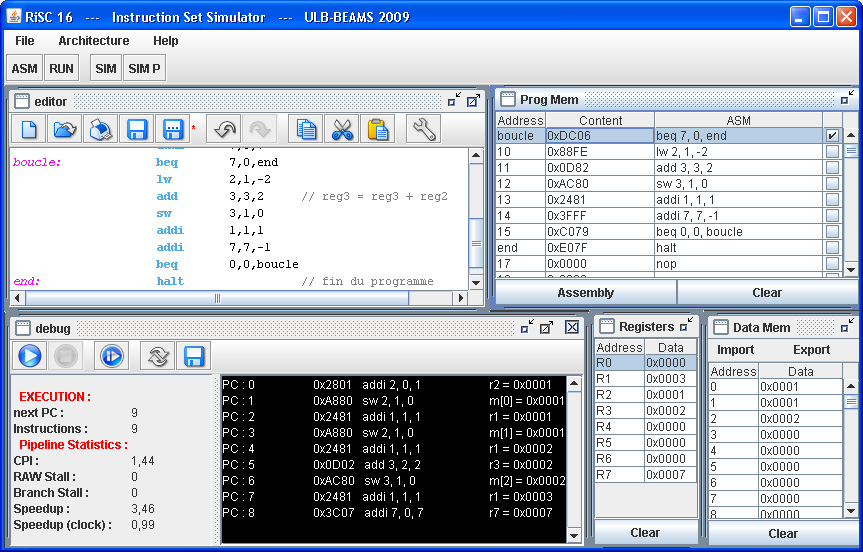
\includegraphics[width=15cm]{100000000000035F000002289D31421E.jpg}
	\end{center}
\caption{Simulator window}
\label{fig:simulator}
\end{figure}

%Présentation de l'interface :
%Le simulateur se compose tout d'abord d'un éditeur à coloration syntaxique. Les labels, les adresses, les commentaires et les instructions disposent ainsi d'une coloration qui leur est propre. En ce qui concerne les instructions, une distinction est faite entre les instructions du RiSC16 original et les instructions ajoutées par la suite. Cette coloration permet en un rapide coup d'œil de vérifier la validité du code assembleur introduit dans l'éditeur.
%Une fois que le programme assembleur est écrit, le bouton "RUN" permet de lancer l'environnement de simulation proprement dit. De nouvelles fenêtres apparaissent :
%une fenêtre contenant la mémoire programme avec le code déjà assemblé ;
%une fenêtre montrant le contenu de la mémoire de données ;
%une fenêtre montrant le contenu des registres ;
%une fenêtre permettant l'exécution de la simulation et affichant un traçage ainsi que des statistiques concernant cette exécution.
%Les trois premières fenêtres sont familières puisqu'elles sont identiques aux affichages des autres simulateurs.
%Voyons  plus en détail le contenu de la dernière fenêtre :
%La dernière fenêtre est constituée de différents boutons :
%PLAY (RUN) : exécute le programme jusqu'à rencontrer un breakpoint ou l'instruction halt.
%STOP : arrête le mode RUN.
%NEXT : mode pas à pas (instruction par instruction).
%RESET : remet le PC à 0, mais ne vide pas le contenu des registres et de la mémoire de données !
%SAVE : permet de sauver la trace dans un fichier texte.
%Elle contient également des statistiques concernant l'exécution du programme :
%CPI : cycles par instruction.
%RAW Stall : nombre d'accidents du type conflit de données suite à une instruction lw.
%Branch Stall : nombre de branchements effectué.
%Speedup : facteur d'accélération du pipeline qui indique de combien la version pipeline est plus rapide par rapport à une version séquentielle hypothétique utilisant le même séquencement de chaque étape d’instruction que le RiSC16 pipe-line soit 70 ½ coups d’horloge (5 étages x 14 ½ coups d’horloge). Speedup = profondeur_du_pipeline / CPI
%Speedup (clock) : indice correspond au gain réel en tenant compte de la durée prise par un cycle dans la version séquentielle du RiSC16 (=10 coups d'horloge) et dans la version pipeline (=7 coups d'horloge). Il est égal à  .
%Enfin, sur la droite de cette fenêtre est affichée la trace.
\newpage
\section{Simulator use}
All parameters defining an architecture are available in the menu ``Architecture". Main parameters are:
\begin{itemize}
\item Instruction set (``Architecture > Instruction set"):
\begin{itemize}
\item RiSC16 original: 8 instructions.
\item Special IS[1]: 8 instructions + 8 new instruction. See Table \vref{tab:IS1}.
\item Special IS[2]: same as IS[1] but \verb!BG! replaced by \verb!MUL!.
\item Other: custom instruction set. Instructions can be selected in a list.
\end{itemize}
\item 8, 16, 32 or 64 registers (``Architecture > Registers")
\item Size of immediate constant fields in instructions can be modified (``Architecture > Imm \& Instru size")
\end{itemize}
These parameters will obviously change the instruction length.
%
It is also possible to specify if instructions use signed or unsigned operands. This choice has an impact on \verb!BL! et \verb!BG! and on the way \textit{overflow} and \textit{carry} are processed for instructions \verb!ADD!, \verb!SUB!, \verb!SHL! and  \verb!SHA!.

Several predefined architecture are available in the ``Architecture > preset" menu:
\begin{itemize}
\item Original RiSC16
\item Special IS[1] -- 8 reg -- 16 17-bit instructions
\item Special IS[1] -- 16 reg -- 16 24-bit instructions, see Table \vref{tab:IS1-16-24}
\item Special IS[2] -- 8 reg -- 16 17-bit instructions, see Table \vref{tab:IS1}, \verb!BG! replaced by \verb!MUL!
\end{itemize}

Once the chosen architecture is selected, configured and the assembly code written, the ``RUN" button compiles the program for the selected architecture. New windows will appear to run the actual simulation.

\newpage
% \section{Manipulation}
% \begin{Q}
% Why isn't the pipeline acceleration factor equal to the pipeline's depth?
% \end{Q}
% \begin{Q}
% Run the example code from lab 1 to instruction \#8 and observe the ``speedup" and ``speedup (clock)". Observe, explain and conclude.
% \end{Q}
% \begin{Q}
% Considering a program without any hazard, what is the number of instructions to execute to make the pipeline more efficient? $T_{\on{pipe}}=7$, $T_{\on{seq}}=10$
% \end{Q}
\subsection{Assignment}

Compare performances of several algorithm using several instruction sets:

\noindent Choose an operator in $\left\lbrace <, >, \leq, \geq \right\rbrace$.

\begin{Q}
	Determine a set of test vectors which could test the functionality and corner cases of your operator. Justify all vectors utility. We target \textbf{signed numbers}.	[1 point]
\end{Q}

\begin{Q}
	Write the code for your operator using:
	\begin{itemize}
	\item the original 8 instructions [1 point]
	\item the Special IS[1] [1 point]
	\end{itemize}
\end{Q}

\begin{Q}

%\begin{itemize}
%\item Write a program which compare (< or >) two signed numbers stored in \reg{1} and \reg{2}. 1 will be written in \reg{3} if the comparison is true, else 0.
%\begin{enumerate}
%\item Write\footnote{\label{assign}And test it using the online verification tool, the results will be included in the quotation of these labs, see Lab4 for more details.} the program using the 8 original instructions
%\item Write\footref{assign} the program using the Special IS[1] instruction set.
%\end{enumerate}
%\item
Write a program to multiply the \textbf{unsigned} content of \reg{1} and \reg{2} and write the result in \reg{3} and \reg{4}, LSB in \reg{3}.
\begin{enumerate}
\item \sout{Write the program using the original instruction set} Already done in Lab 1, lucky you!
\item Write\footnote{\label{assign}And test it using the online verification tool, the results will be included in the quotation of these labs.} the program using the Special IS[1] instruction set. [3 points]
\item Write\footref{assign} the program using the Special IS[2] and using the \verb!MUL! instruction. [3 points]
\item Conclude. [1 point]
\end{enumerate}
Note : the processor uses signed integers (complement to 2 representation) by default.
%\end{itemize}
\end{Q}

\end{document}



%



Utilisation du programme

L'ensemble des paramètres définissant une architecture sont accessibles via le menu Architecture. Passons-les en revue.
Le premier choix concerne la sélection du jeu d'instructions (Architecture > Instruction Set).
RiSC16 original et ses 8 instructions.
Special IS[1] = 8 instructions de base + 8 nouvelles instructions (voir tableau Special IS[1] en première page)
Special IS[2] : idem que Special IS[1] sauf que bg est remplacé par mul
Other : permet d'avoir un jeu d'instructions personnalisé en sélectionnant les instructions que l'on souhaite utiliser.
Il est possible de choisir entre 8, 16, 32 ou 64 registres (Architecture > Registers).
La taille des champs contenant les valeurs immédiates peut être modifiée (Architecture > Imm & Instru Size).
Ces différents paramètres auront une incidence sur la longueur des instructions.

Enfin, il est également possible de déterminer si les opérations agissent sur des nombres signés ou des nombres non-signés. Ce choix aura une influence sur les opérations bl (branch if lower) et bg (branch if greater) et indiquera également la manière de calculer les débordements pour les instructions add, sub, shl, sha (overflow en arithmétique signée et carry en arithmétique non-signée).

Certaines présélections sont disponibles via le menu (Architecture – Preset)
RiSC16 original qui correspond à la configuration de base.
Special IS[1] – 8 reg – Instruction 17 bits : 8 instructions de base + 8 nouvelles instructions et gestion des overflow
Special IS[1] – 16 reg – Instruction 24 bits : voir tableau en page 2
Special IS[2] – 8 reg – Instruction 17 bits : voir tableau en page 1 mais l'instruction bg est remplacée par l'instruction mul

Une fois que l'architecture ciblée a été sélectionné et que le programme assembleur est écrit, le bouton "RUN" permet de compiler le programme en utilisant le jeu d'instructions sélectionné. De nouvelles fenêtres vont apparaitre pour permettre de lancer la simulation à proprement parler.
Manipulation
1. Pourquoi le facteur d’accélération du pipeline (speedup) n’est pas égal à la profondeur du pipeline?
2. Exécutez le programme d’exemple jusque l’instruction 8 et observez le « speedup » et le « speedup (clock) ». Que constatez-vous? Expliquez votre observation.
3. Si l’on considère un programme où aucun accident de dépendance ou de contrôle ne se produit, quel est le nombre d’instructions qui doit être exécuté pour que le pipe-line prenne l’avantage compte tenu des temps d’exécution d’un cycle : Tpipe = 7 et Tseq = 10
4. Comparer les performances d'algorithmes en utilisant différents jeux d'instruction. Pour ce faire :
Écrirez un programme qui compare (> ou <) deux nombres signés situés dans les registres 1 et 2. Un 1 sera écrit dans le registre 3 si la comparaison est vérifiée et un 0 dans le cas contraire.
Écrire ce programme en utilisant les 8 instructions de base.
Écrire ce programme en utilisant le jeu d'instruction évolué (Special IS[1])
Écrirez un programme qui multiplie le contenu des registres 1 et 2 et place le résultat dans les registres 3 et 4 (mot de poids faible dans le registre 3).
Écrire ce programme en utilisant les 8 instructions de base.
Écrire ce programme en utilisant le jeu d'instruction évolué (Special IS[1]).
Écrire ce programme en utilisant un jeu d'instructions comprenant l'instruction mul (Special IS[2]).


\end{document}
This lab is about the internal behaviour of a RISC processor and goals are:
\begin{itemize}
\item understand internal behaviour of a simple pipelined processor, especially pipeline hazards
\item write and test some programs in assembly code for this specific RISC processor and compare performances and implementation  with version from Lab 1
\item watch this code running in a simulation
\end{itemize}


%Les buts de cette manipulation sont :
%de comprendre les principes liés à une architecture en pipeline, en particulier la gestion des accidents (pipeline hazards),
%de comparer les deux architectures en termes de performance et de mise en œuvre.
To reach these goals, you will use another simulator for the pipelined version of the RiSC16 initially designed by Bruce Jacob. The processor has exactly the same features that the sequential version but is implemented using a 5-stage pipeline. Several blocks were added, as shown on figure \vref{fig:risc}.

\begin{figure}[h!]
	\begin{center}
		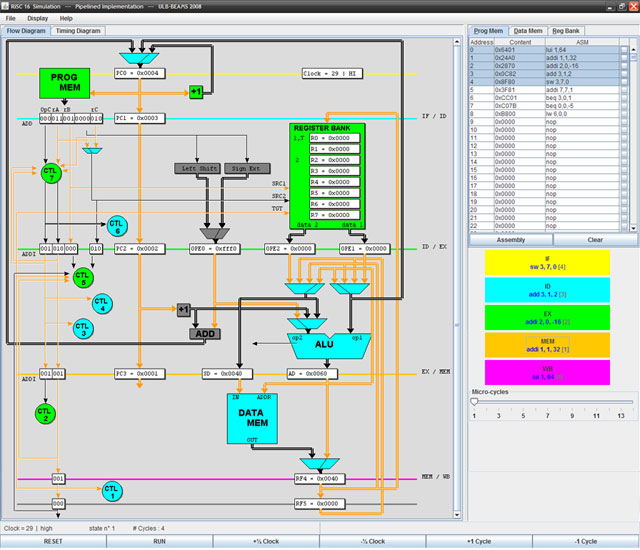
\includegraphics[width=15cm]{figures/100000000000028000000226ACEB2984.jpg}
	\end{center}
\caption{Pipelined RiSC-16 processor}
\label{fig:risc}
\end{figure}

The pipeline has 5 stages and instructions are splitted into:
\begin{enumerate}
\item \textbf{IF} (Instruction Fetch): instruction is read from program memory. \verb!PC! is also incremented.
\item \textbf{ID} (Instruction Decode): opcode is decoded and operands for ALU are read in the register bank
\item \textbf{EX} (EXecute): ALU processes the operation
\item \textbf{MEM} (MEMory): access to Data memory
\item \textbf{WB} (Write-Back): result is written in register
\end{enumerate}
%Pour cela, nous utiliserons un autre simulateur qui permet d’exploiter la version pipeline du RiSC16 décrit par le professeur Bruce Jacob. Les caractéristiques (instructions, nombre de registres, …) sont identiques à la version séquentielle. Mais, comme on peut le voir sur la figure ci-dessous, le nombre de blocs et de bus est plus élevé dans une architecture de ce type.
%Il s’agit d’un pipeline de 5 étages et l’exécution d’une instruction est décomposée de la manière suivante :
%IF (Instruction Fetch) : étape pendant laquelle l’instruction est lue dans la mémoire d’instruction. Le Program Counter est également incrémenté.
%ID (Instruction Decode) : étape pendant laquelle l’opcode est décodée et les opérandes de l’ALU sont lues dans le banc de registres.
%EX (EXecute) : étape pendant laquelle l’ALU effectue l’opération.
%MEM (MEMory) : étape durant laquelle on accède à la mémoire donnée.
%WB (Write-Back) : étape durant laquelle le résultat est placé en registre.
%Toutes les étapes ont une durée d’un cycle.
%L’interface a été volontairement calquée sur le simulateur séquentiel, pour passer facilement de l’un à l’autre.


All stages are completed in one clock cycle. The interface presented in the simulator is designed in the same way that the sequential version to ease switching between the two implementations.

There are several zones in the simulator window:
\begin{itemize}
\item The execution zone has two tabs:
\begin{itemize}
\item The first one shows the different steps of a cycle
\item The second one shows the cycle-instruction diagram (see figure \vref{fig:pipe}). The number of cycles per instruction (CPI) is also shown.
\end{itemize}
%this gives the result:\\
\begin{figure}[h!]
	\begin{center}
		\begin{tabular}{r *{5}{C{1cm}}}
\toprule
  	Stage:			& 1	& 2 & 3 & 4 & 5 \\
 \midrule
\color{blue}lui 1, 64 \color{red}[0] 	& \cellcolor{yellow}IF& \cellcolor{cyan}ID & \cellcolor{green}EX &  \cellcolor{orange}MEM & \cellcolor{purple}WB \\
\color{blue}addi 1, 1, 32 \color{red}[1] 	&  	& \cellcolor{yellow}IF & \cellcolor{cyan}ID &  \cellcolor{green}EX & \cellcolor{orange}MEM \\
\color{blue}addi 2, 0, -16 \color{red}[2] &   &   & \cellcolor{yellow}IF & \cellcolor{cyan}ID & \cellcolor{green} EX \\
\color{blue}add 3, 1, 2 \color{red}[3] 	&  	&   &   & \cellcolor{yellow}IF & \cellcolor{cyan}ID \\
\color{blue}sw 3, 7, 0 \color{red}[4] 	&   &   &   &   & \cellcolor{yellow}IF \\
\bottomrule
\end{tabular}
	\end{center}
\caption{Pipeline execution}
\label{fig:pipe}
\end{figure}

\item The memory zone on the right has 3 tabs to show and edit content of program memory, data memory and file register.
\item Another zone on the right details the content of the pipeline for each stage and the cursor shows the current step of the cycle.
\item The lower part groups the interaction possibilities: buttons provide reinitialisation (reset), execution (run), instruction execution and undo last clock-cycle capabilities.
\item The central zone shows the blocks for this architecture.
\end{itemize}

As far as the internal blocks of the processor are concerned, two particularities occur:
\begin{enumerate}
\item The control unit is split into several smaller units. Each one has a specific role either for a flawless execution or for managing pipeline hazards.
\item Between each stages, Pipeline registers were added to store states variables related to the current stage. Among these variables, we can find the opcode, address of registers, state of the \verb!PC!\dots
\end{enumerate}
Thanks to these registers the pipeline can work as expected because they are the link between stages.

Only pipeline registers and control unit are synchronous. Other blocks are asynchronous.

The figure \vref{fig:seq} shows the execution sequence of instructions.
\begin{figure}[h!]
\setlength{\tabcolsep}{3pt} %no extra space in cells to keep constant tabular width
\footnotesize
	\begin{center}
%		\includegraphics[width=15cm]{figures/-crop.pdf}
\begin{tabular}{r|*{2}{C{0.5cm}}|*{2}{C{0.8cm}}|cC{1.3cm}|C{0.8cm}c|c|c|c|C{1.5em}|C{0.5cm}C{0.5cm}}
\toprule
 & 1 & 2 & 3 & 4 & 5 & 6 & 7 & 8 & ~9 & 10 & 11 & 12 & 13 & 14 \\
 \midrule
%\cellcolor{yellow}Fetch & \multicolumn{2}{c}{\cellcolor{yellow}+1,ROM} & \cellcolor{yellow}ROM  &   &   &   &   &   &   &   &   &   & \multirow{5}{*}{\multicolumn{2}{C{2cm}}{\cellcolor{lightgray}Pipeline register update}} \\
%\cellcolor{cyan}Decode & \multicolumn{2}{C{1.5cm}}{\cellcolor{cyan}CTL7, \newline LS, SE, \newline RF(src1)} & \cellcolor{cyan}RF(src1) &   & \multicolumn{2}{C{1.5cm}}{\cellcolor{cyan}CTL6} & \multicolumn{2}{C{2cm}}{\cellcolor{cyan}MUXs2,\linebreak MUXOPE0} & \multicolumn{3}{c}{\cellcolor{cyan}RF(src2)}&  & \multicolumn{2}{C{2cm}}{\cellcolor{lightgray}Pipeline register update} \\
%
%\cellcolor{green}Execute & \multicolumn{2}{C{1.5cm}}{\cellcolor{green}CTL5, (+1)} & \multicolumn{2}{C{2cm}}{\cellcolor{green}CTL4,\linebreak ADD,\linebreak MUXalu1, MUXalu2} &  \multicolumn{2}{C{1.5cm}}{\cellcolor{green}CTL3, MUXop2} & \multicolumn{2}{c}{\cellcolor{green}ALU} & \multicolumn{2}{c}{\cellcolor{green}CTL3} & \multicolumn{2}{c}{\cellcolor{green}MUXpc} & \multicolumn{2}{C{2cm}}{\cellcolor{lightgray}Pipeline register update} \\
%
%\cellcolor{orange}Memory & \multicolumn{2}{c}{\cellcolor{orange}CTL2} & \multicolumn{2}{c}{\cellcolor{orange}RAM} & \multicolumn{1}{C{1.5cm}}{\cellcolor{orange}RAM, \linebreak CTL2} & \cellcolor{orange}CTL2 & \multicolumn{2}{c}{\cellcolor{orange}MUXrf4} &   &   &   &   & \multicolumn{2}{C{2cm}}{\cellcolor{lightgray}Pipeline register update} \\
%\cellcolor{purple}Write Back &   &   & \multicolumn{2}{c}{\cellcolor{purple}CTL1} & \multicolumn{3}{c}{\cellcolor{purple}RF} &   &   &   &   &  & \multicolumn{2}{C{2cm}}{\cellcolor{lightgray}Pipeline register update} \\
\cellcolor{yellow}Fetch & \multicolumn{2}{|c|}{\cellcolor{yellow}+1,ROM} & \cellcolor{yellow}ROM  &   &   &   &   &   &   &   &   &   & \cellcolor{lightgray} & \cellcolor{lightgray} \\%\multicolumn{2}{c}{Pipeline register update}} \\
%\multirow{4}{2cm}{\multicolumn{2}{c}{Pipeline register update}}
\cellcolor{cyan}Decode & \multicolumn{2}{|C{1.3cm}|}{\cellcolor{cyan}CTL7, \newline LS, SE, \newline RF(src1)} &  \cellcolor{cyan}RF (src1) &   & \multicolumn{2}{|C{1.3cm}|}{\cellcolor{cyan}CTL6} & \multicolumn{2}{|C{1.6cm}|}{\cellcolor{cyan}MUXs2,\linebreak MUXOPE0} & \multicolumn{3}{|c|}{\cellcolor{cyan}RF(src2)}&  & \cellcolor{lightgray} &\cellcolor{lightgray} \\
%
\cellcolor{green}Execute & \multicolumn{2}{|C{1.3cm}|}{\cellcolor{green}CTL5, (+1)} & \multicolumn{2}{|C{1.8cm}|}{\cellcolor{green}CTL4,\linebreak ADD,\linebreak MUXalu1, MUXalu2} &  \multicolumn{2}{|C{1.3cm}|}{\cellcolor{green}CTL3, MUXop2} & \multicolumn{2}{|c|}{\cellcolor{green}ALU} & \multicolumn{2}{|c|}{\cellcolor{green}CTL3} & \multicolumn{2}{|c|}{\cellcolor{green}MUXpc} &\cellcolor{lightgray} &\cellcolor{lightgray}  \\
%
\cellcolor{orange}Memory & \multicolumn{2}{|c|}{\cellcolor{orange}CTL2} & \multicolumn{2}{|c|}{\cellcolor{orange}RAM} & \multicolumn{1}{|C{1.3cm}|}{\cellcolor{orange}RAM, \linebreak CTL2} & \cellcolor{orange}CTL2 & \multicolumn{2}{|c|}{\cellcolor{orange}MUXrf4} &   &   &   &  & \cellcolor{lightgray} & \cellcolor{lightgray} \\
\cellcolor{purple}Write Back &   &   & \multicolumn{2}{|c|}{\cellcolor{purple}CTL1} & \multicolumn{3}{|c|}{\cellcolor{purple}RF} &   &   &   &   & & \multicolumn{2}{c}{\multirow{-10}{1.2cm}{\cellcolor{lightgray}\centering Pipeline register update}} \\
\bottomrule
\end{tabular}
	\end{center}
\caption{Instruction sequencing}
\label{fig:seq}
\end{figure}

The architecture performance can be measures using the cycles per instruction (CPI).

An ideal CPI for a pipeline should be 1 after each cycle, that means that an instruction ends at each cycle.

But actually, the pipeline is subject to hazards. In this RiSC16 architecture, only dependency conflicts (Data hazards) and control problems (Control Hazards) can occur.

\subsection{Dependency hazards}
Dependency conflicts happens when an instruction needs a result from a previous instruction which is not completed yet. Only incidents of type ``Read After Write" can happen in the RiSC16.
To solve this problem, several possibilities exist:
\begin{itemize}
\item Data forwarding: a value is taken from a previous stage before its written in the register bank and is used as input to the ALU. Thanks to this mechanism, there is no penalty. Data forwarding is signalled by a message in the simulator.
\item When the \verb!LW! instruction is in stage EX and an instruction in ID stage uses an operand at the same address than the destination register for the LW instruction, a Data hazards occurs. This hazard cannot be solved using Data forwarding, the only way to solve the issue is to stall the pipeline and so add a "bubble". This will add a penalty of one cycle. This is signalled by a stall event in the simulator.
\end{itemize}
%On peut distinguer plusieurs zones sur la capture d'écran ci-dessus :
%la zone d'exécution au centre contenant 2 onglets :
%le 1er permet d'observer le déroulement des différentes étapes d'un cycle ;
%le 2ème permet d'afficher le diagramme cycle-instruction (voir ci-dessous). Le nombre de cycles par instruction (CPI)  est également indiqué.

%la zone "Mémoires" sur la droite contient 3 onglets permettant de voir et d’éditer le contenu de la mémoire programme, de la mémoire de données et du banc de registres.
%une autre zone sur la droite permettant de connaître à chaque instant l’instruction présente dans chaque étage du pipeline et le curseur permet de voir où l’on se situe dans le cycle.
%la zone inférieure contient les boutons permettant d’interagir avec le simulateur. Les boutons ± 1 cycle permettent d'avancer ou de reculer d'un étage de pipeline.
%Au niveau des blocs constituant cette architecture, signalons deux particularités :
%l’unité de contrôle est éclatée en plusieurs petites unités distinctes. Chacune ayant un rôle bien spécifique relatif au déroulement normal du processeur ou à la gestion des différents accidents pouvant se produire dans un pipeline.
%entre chaque étage, se trouvent des registres (Pipeline Registers) qui ont pour rôle de stocker les variables d'état relatives à l’instruction en cours dans l’étage. Parmi ces variables d'état, citons pour exemple l’opcode, les adresses des différents registres, l’état du PC, …
%C’est grâce à ces registres que le pipeline peut progresser, car ils sont le lien entre les différents étages.
%Seuls les Pipeline Registers et les unités de contrôle sont synchronisés. Les autres éléments réagissent dès que leurs entrées sont actives ou que leur signal de contrôle a été reçu.
%La figure suivante montre le séquencement des événements durant un cycle machine. Chaque étape prenant le même temps d’exécution, elles ont toutes été alignées sur la plus longue.

%La performance d’une architecture peut être mesurée à partir du nombre de cycles par instruction (CPI).
%Le CPI idéal d’un pipeline en régime serait égal à 1 car après chaque cycle, une instruction sortira du pipeline.
%Mais, le pipeline est sujet à un certain nombre d’accidents (hazards). Les seuls accidents pouvant se produire dans l'architecture RISC16 sont les conflits de dépendance (Data Hazards) et les problèmes de contrôle (Control Hazards).
%Les conflits de dépendance se produisent lorsqu’une instruction requiert le résultat d’une instruction précédente, alors que celle-ci ne peut pas encore le fournir. Seuls les accidents de type RAW (Read After Write) peuvent se produire ici. Les mécanismes de résolution pour ce type d’accidents sont les suivants :
%le Data Forwarding permet de prélever une valeur dans les étages précédents (situés plus bas sur le flow diagram du simulateur) avant qu’elle ne soit écrite dans le banc de registre et de l’utiliser comme opérande à l’entrée de l’ALU. Grâce à ce mécanisme, il n’y a aucune pénalité. Au cours de l'exécution par le simulateur, le Data Forwarding est signalé par un message d'information.
\subsection{Control conflicts}
Control conflicts happens because of branch and call procedures. The address of the next instruction is computed in the execute stage an so, when a jump occurs, instructions loaded in the 2 previous stages are irrelevant and are discarded. This accident add a penalty of 2 cycles and is name stomp event in the simulator.

Various information messages are displayed when an accident occurs. They can be disabled using the "Display > Alerts" menu.

\clearpage\newpage
\section{Manipulation}
\begin{Q}
Reuse the example of the first lab and draw the cycle-instruction diagram for the 25 first cycles. Compare the result with the simulation. Beware, accidents happen in simulation.
\end{Q}
\begin{Q}
What is the function of each control unit? Which ones are used during accidents solving?
\end{Q}

\begin{Q}
Correct the program to suppress data hazards.
\end{Q}

%lorsque l’instruction LW se trouve au niveau de l’étape EX et que l’instruction se trouvant dans l’étape ID utilise un opérande situé à la même adresse que la destination de l’instruction LW, il y a également un conflit de dépendance de données, qui ne peut pas être solutionné directement au moyen du Data Forwarding. La seule solution à ce problème est de bloquer le pipeline. Ce blocage entrainera la création d’une bulle et il y aura une pénalité d’1 cycle. Dans le simulateur, cet événement porte le nom de stall event.

%Les conflits de contrôle sont liés aux branchements et appels de procédure. Le calcul de l’adresse de la prochaine instruction se déroule dans l’Execute Stage et donc, en cas de saut dans le programme, les instructions chargées dans les deux étages précédents deviennent inutiles et sont donc supprimées. Cet accident entraine une pénalité de 2 cycles. Dans le simulateur, cet événement porte le nom de stomp event.
%Des messages d’informations apparaissent lorsqu’un accident se produit. Ceux-ci peuvent être désactivés dans le menu "Display > Alerts".
%Manipulation

%Reprenez l’exemple de la manipulation 1. Prédisez le diagramme (Cycle | Instruction) pour les 25 premiers cycles et comparez ensuite avec le résultat de la simulation. Soyez attentif au déroulement de la simulation, en particulier à l’approche d’accidents.
%Quelle est la fonction de chacune des unités de contrôle et quelles sont celles jouant un rôle dans la prévention des accidents?
%Corrigez le programme pour supprimer les conflits de dépendance de données entraînant une pénalité.
\begin{Q}
Observe the CPI at the end of program execution and compare with the result of first lab.
\end{Q}

\begin{Q}
Find a way to compute the CPI using:
\begin{itemize}
\item pipeline $\on{depth}$ (here : 5)
\item instruction fully executed: $\on{instruction}$
\item number of stall events: $\on{stall}$
\item number of stomp events: $\on{stomp}$
\end{itemize}
\end{Q}

\begin{Q}
How would you modify the hardware to improve the design?
\end{Q}

\begin{Q}
Complete the program of first lab (multiplication of two registers).
\end{Q}

\end{document}





Observez le CPI obtenu à la fin de l’exécution du programme et constatez le gain par rapport à l’architecture utilisée la semaine dernière.
Trouvez la formule permettant de calculer le CPI et liant les variables suivantes :
Profondeur du pipeline : depth (=5)
Nombre d’instructions exécutées complètement : instruction
Nombre de stall event : stall
Nombre de stomp event : stomp
Quelle(s) amélioration(s) hardware pourrai(en)t encore améliorer ce design?
Terminez le labo précédent : écrire un programme qui multiplie le contenu de deux registres.
Annexe : Programme d'exemple

		addi 	2,0,1
		sw   	2,1,0
		addi 	1,1,1
		sw   	2,1,0
		addi 	1,1,1
		add  	3,2,2
		sw   	3,1,0
		addi 	1,1,1
		addi 	7,0,7
boucle: 		beq  	7,0,end
		lw	2,1,-2
		add 	3,3,2
		sw   	3,1,0
		addi 	1,1,1
		addi 	7,7,-1
		beq  	0,0,boucle
end: 		halt



\end{document}

This lab is about the internal behaviour of a RISC processor and goals are:
\begin{itemize}
\item understand internal behaviour of a simple processor
\item write and test some programs in assembly code for this specific RISC processor
\item watch this code running in a simulation
\end{itemize}

You will use a RISC16 processor which is a RISC processor developped for teaching by \textsc{Bruce Jacob} (University of Maryland) for a course about microelectronics.
This processor based on a Harvard architecture works on 16bit data and instructions. 8 instructions, one 8register bank, 216word RAM and ROM are available.

%Fonctionnement interne d'un processeur RISC (1/3)
%Introduction
%Les buts de cette manipulation sont :
%illustrer le fonctionnement interne d'un processeur simple,
%vous faire programmer en assembleur un processeur de type RiSC.
%Pour cela, nous utiliserons un programme de simulation qui permet d'observer le fonctionnement interne du processeur RiSC-16. C'est un processeur RISC, développé dans un but didactique par le professeur Bruce Jacob de l'université du Maryland, dans le cadre d'un cours de microélectronique :
%il manipule des données et des instructions codées sur 16 bits,
%il n'a que huit instructions,
%il possède un banc de huit registres, une rom et une ram de 216 mots de 16bits,
%son architecture est de type Harvard.

The simplicity of the instruction set allows a quick learning curve and is enough to address complex problems.

The internal structure of the processor is simple enough to be represented in a didactic way like on Figure \vref{fig:RISC}.

%Son jeu d'instruction réduit permet une prise en main rapide tout en étant assez complet pour résoudre des problèmes complexes.
%La structure interne du RiSC-16 est suffisamment simple pour être représentée et affichée sur un écran d'ordinateur, comme le montre la capture d'écran ci-dessous :
\begin{figure}[h!]
	\begin{center}
		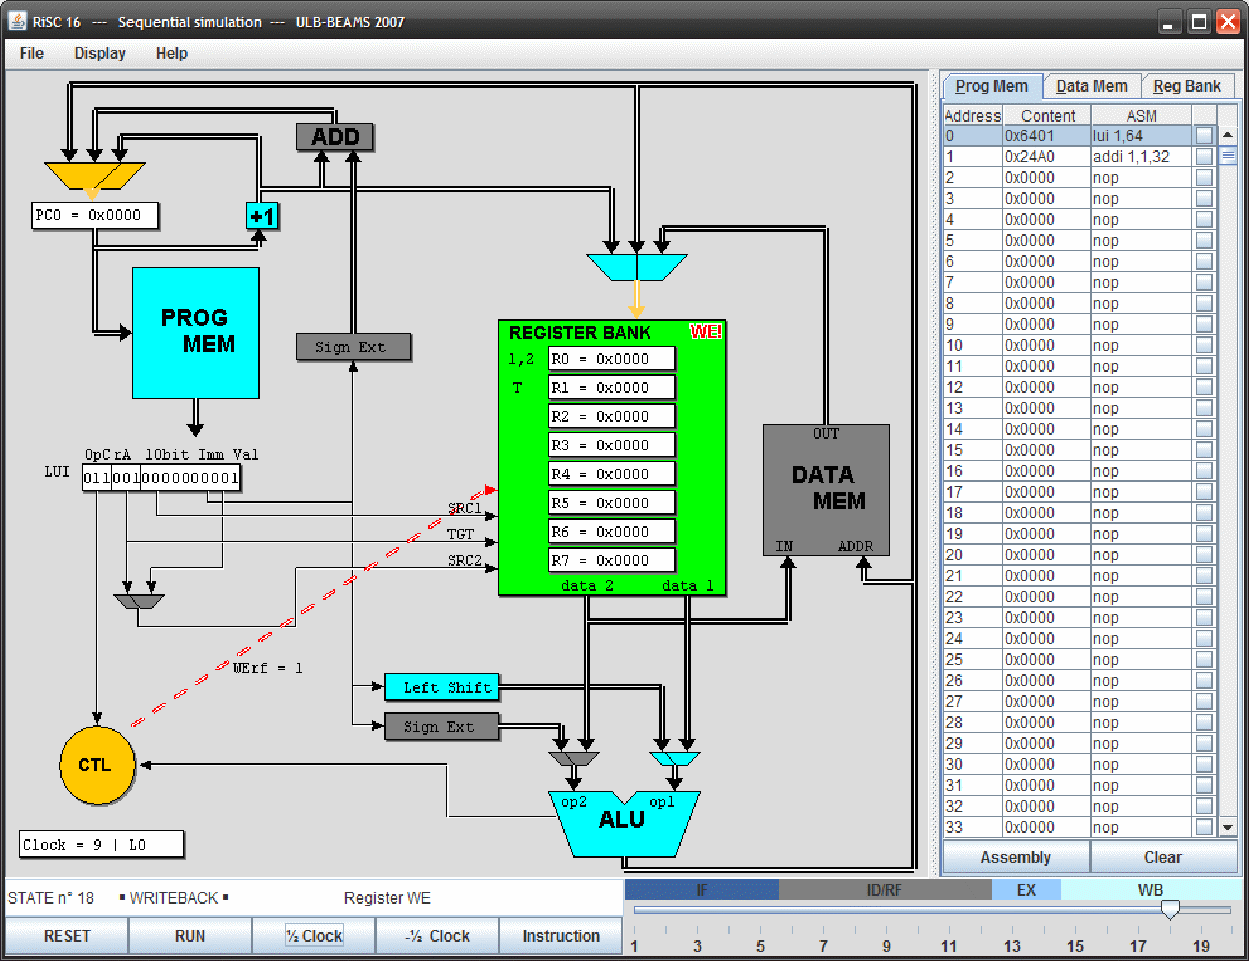
\includegraphics[width=15cm]{RiSC16_enonce_1_html_m16049efd.png}
	\end{center}
\caption{RISC16 -- Simulation view}
\label{fig:RISC}
\end{figure}
%
The user interface has 4 zones:
\begin{itemize}
\item The lower part groups the interaction means: buttons provide reinitialisation (reset), execution (run), half-cycle execution, instruction execution and undo last instruction capabilities.
\item The text zone above displays general informations about instruction execution. The cursor on the right can be used to follow each step of instruction execution and can be used to jump at any step of this instruction.
\item The zone on the right shows and allows editing program and data memory. A third tab shows register, they can also be modified.
\item The central zone shows the microprocessor representation

\end{itemize}

%Au niveau de l’interface du simulateur, on distingue 3 zones :
%la zone inférieure comprend les différents moyens d’interaction. Les boutons permettent de réinitialiser l’état du processeur (reset), d’exécuter un programme jusqu’au prochain breakpoint (run), d’exécuter le programme par demi-coups d’horloge ou par instruction, d’annuler le dernier demi-coup d’horloge.

%La zone de texte située juste au-dessus des boutons affiche les grandes lignes de ce qu’il se passe durant l’exécution de l’instruction. Le curseur sur la droite permet de suivre l’exécution d’une instruction au cours du temps et de revenir à n'importe quel moment de cette exécution ;

%la zone sur la droite permet de voir et d’éditer le contenu de la mémoire programme et de la mémoire de donnée. Un troisième onglet permet de modifier le contenu des registres ;

%la zone centrale comprend la représentation du microprocesseur.

%

\section{Processor description}

Several blocs are used in this microprocessor:
\begin{itemize}
\item Program memory (\verb!PROG MEM!) and Data memory (\verb!DATA MEM!) --because of the Harvard architecture
\item Internal register bank (\verb!Register Bank!) to store operands and computation results. \verb!Register 0! has a special meaning: it's a read only register containing the \verb!0! value. A write in register 0 has no effect.
\item The Arithmetic and Logic Unit is used to execute the operations needed to execute instructions. 4 operations are possible:
	\begin{enumerate}
	\item add two operands, used during \verb!ADD, ADDI, LW, SW!
	\item bitwise NAND of two operands, used obviously during \verb!NAND!
	\item no modification, result is \verb!OP1!, used during \verb!LUI, JALR!
	\item operand comparison, used during \verb!BEQ!
	\end{enumerate}
\item The Control Unit (\verb!CTL!) decodes the opcode and configure other locks accordingly. It's synchronised on the clock and can be used for rising edge or falling edge operation.
\item The program counter \verb!PC0!
\item The instruction register
\item The incrementer \verb!+1!
\item The adder (\verb!ADD!) to compute the address for jumps (Branch with \verb!BEQ!)
\item The immediate value converter (left shift and sign extension)
\end{itemize}

Blocks and linked together using buses with width of 1, 3, 6, 10 or 16 bits. Control signals are:
\begin{itemize}
\item \verb!WE_rf!: write in register bank
\item \verb!FUNC_alu!: operation to use
\item \verb!Mux_rf!, \verb!Mux_alu! (1,2), \verb!Mux_tgt!, \verb!Mux_pc! : select multiplexer input
\item \verb!WE_dmem!: write in data memory
\item \verb!PSEN! : read from program memory.
\item \verb!WE_PCO! : write data into \verb!PC0!.
\end{itemize}


%Détaillons les différents blocs constituant ce microprocesseur :
%la mémoire programme (PROG MEM) et la mémoire de données (DATA MEM) séparées, puisque c'est une architecture de Harvard ;
%le banc de registres internes (Register Bank) pour stocker les opérandes et les résultats des opérations; une particularité de ce banc de registres est que le registre 0 contient toujours 0 (une écriture dans ce registre n'a aucun effet);
%l'unité arithmétique et logique (ALU) pour exécuter les différentes opérations nécessaires à l'exécution des instructions. Ces opérations sont au nombre de 4 : addition des deux opérandes (ADD, ADDI, LW et SW), NAND bit à bit des deux opérandes (NAND), passage sans modification de l'opérande op1 (LUI et JALR) et comparaison des deux opérandes (BEQ);
%l’unité de contrôle (CTL) qui s’occupe de décoder l’opcode et de commander les autres blocs en leur envoyant des signaux de contrôle. Elle est synchronisée sur l’horloge et peut activer un signal de contrôle sur un flanc montant comme sur un flanc descendant.
%le Program Counter (PC0);
%le registre d'instruction (en dessous de la mémoire programme);
%l'incrémenteur (+1), qui incrémente le Program Counter dans le cas du déroulement séquentiel du programme;
%l'additionneur (ADD), qui calcule l'adresse dans le cas d'un branchement (BEQ);
%les blocs de conversion de valeurs immédiates (left shift et sign ext).
%Les différents blocs sont reliés entre eux par des bus pouvant avoir des tailles de 1, 3, 6, 10 ou 16 bits. Les différents signaux de contrôle sont :
%WE_rf : ordre d'écriture dans le banc de registre
%FUNC_alu : pour indiquer à l'ALU quelle opération effectuer
%Mux_rf, Mux_alu (1,2), Mux_tgt, Mux_pc : sélection de l'entrée active de chaque multiplexeur
%WE_dmem : ordre d'écriture dans la mémoire de données.
%PSEN : ordre de lecture en mémoire de programme.
%WE_PCO : ordre d'écriture dans PC0 de la donnée présente à son entrée.

The instruction set has 8 elementary instructions. None of them can be replaced by any combination of other instructions and complex problems can be solved using only these 8 instructions.
This architecture is RISC at its fate.

\subsection{Instruction detailed description}
Each instruction and how to code it are described below.

\subsubsection{$\on{ADD} : R\left[ \on{regA} \right] \longleftarrow R\left[ \on{regB} \right] + R\left[ \on{regC} \right] $}
\begin{center}
	\begin{tabular}{b{1.2cm}p{8cm}}
	bits & %first line
	 \begin{tabular}{C{1.5cm}C{1.5cm}C{1.5cm}C{2cm}C{1.5cm}}
		3 & 3 & 3 & 4 & 3 \\
	 \end{tabular} 	 \\
	 %second line:
	ADD &
	 \begin{tabular}{|C{1.5cm}|C{1.5cm}|C{1.5cm}|C{2cm}|C{1.5cm}|}
	 	\hline  000 & regA & regB & 0000& regC \\  \hline
	 \end{tabular} \\
	\end{tabular}
\end{center}

Add content from \reg{B} with content from \reg{C} and write result in \reg{A}.


\subsubsection{$\on{ADDI} \on{(ADD\; immediate)} : R\left[ \on{regA} \right] \longleftarrow R\left[ \on{regB} \right] + \on{inned} $}
\begin{center}
	\begin{tabular}{m{1.2cm}m{8cm}}
	bits & %first line
	 \begin{tabular}{C{1.5cm}C{1.5cm}C{1.5cm}C{3.5cm}}
		3 & 3 & 3 & 7 \\
	 \end{tabular} 	 \\
	 %second line:
	ADDI &
	 \begin{tabular}{|C{1.5cm}|C{1.5cm}|C{1.5cm}|C{3.5cm}|}
	 	\hline  001 & regA & regB & signed immediate \\  \hline
	 \end{tabular} \\
	\end{tabular}
\end{center}

Add content from \reg{B} with an immediate 7bit signed constant (-64 to 63) extended to 16bits. Result is written in \reg{A}.

\subsubsection{$\on{NAND} : R\left[ \on{regA} \right] \longleftarrow \on{NOT}\left( R\left[ \on{regB} \right] \& \on{immed}\right) $}
\begin{center}
	\begin{tabular}{m{1.2cm}m{8cm}}
	bits & %first line
	 \begin{tabular}{C{1.5cm}C{1.5cm}C{1.5cm}C{2cm}C{1.5cm}}
		3 & 3 & 3 & 4 & 3 \\
	 \end{tabular} 	 \\
	 %second line:
	NAND &
	 \begin{tabular}{|C{1.5cm}|C{1.5cm}|C{1.5cm}|C{2cm}|C{1.5cm}|}
	 	\hline  010 & regA & regB & 0000 & regC \\  \hline
	 \end{tabular} \\
	\end{tabular}
\end{center}

Bitwise NAND using content from \reg{B} and \reg{C}. Result is written in \reg{A}.

\subsubsection{$\on{LUI} \on{(Load Upper Immediate)} : R\left[ \on{regA} \right] \longleftarrow \on{immed} \& \on{0xFFC0} $}
\begin{center}
	\begin{tabular}{m{1.2cm}m{8cm}}
	bits & %first line
	 \begin{tabular}{C{1.5cm}C{1.5cm}C{5cm}}
		3 & 3 & 10 \\
	 \end{tabular} 	 \\
	 %second line:
	LUI &
	 \begin{tabular}{|C{1.5cm}|C{1.5cm}|C{5cm}|}
	 	\hline  011 & regA & immediate (0 to 0x3FF) \\  \hline
	 \end{tabular} \\
	\end{tabular}
\end{center}

Immediate 10bit constant sign extendted and written in \reg{A}.

\subsubsection{$\on{LW} \on{(Load Word)} : R\left[ \on{regA} \right] \longleftarrow \on{Mem}\left[ R\left[ \on{regB} \right] +immed \right] $}
\begin{center}
	\begin{tabular}{m{1.2cm}m{8cm}}
	bits & %first line
	 \begin{tabular}{C{1.5cm}C{1.5cm}C{1.5cm}C{5cm}}
		3 & 3 & 3 & 7 \\
	 \end{tabular} 	 \\
	 %second line:
	LW &
	 \begin{tabular}{|C{1.5cm}|C{1.5cm}|C{1.5cm}|C{5cm}|}
	 	\hline  100 & regA & regB & signed immediate \\  \hline
	 \end{tabular} \\
	\end{tabular}
\end{center}

Read a word in memory at address (\reg{B}+immediate). Immediate 7bit constant is sign extended to 16bit before the addition. This is an indirect addressing with offset.

\subsubsection{$\on{SW} \on{(Store Word)} : R\left[ \on{regA} \right] \longrightarrow \on{Mem}\left[ R\left[ \on{regB} \right] +immed \right] $}
\begin{center}
	\begin{tabular}{m{1.2cm}m{8cm}}
	bits & %first line
	 \begin{tabular}{C{1.5cm}C{1.5cm}C{1.5cm}C{5cm}}
		3 & 3 & 3 & 7 \\
	 \end{tabular} 	 \\
	 %second line:
	SW &
	 \begin{tabular}{|C{1.5cm}|C{1.5cm}|C{1.5cm}|C{5cm}|}
	 	\hline  101 & regA & regB & signed immediate \\  \hline
	 \end{tabular} \\
	\end{tabular}
\end{center}

Write the content of \reg{A} to memory at address (\reg{B}+immediate). Immediate 7bit constant is sign extended to 16bit before the addition. This is an indirect addressing with offset.


\subsubsection{$ \on{BEQ} \on{(Branch\;if\; EQual)}$ :\\ $\on{if} R\left[ \on{regA} \right]== R\left[ \on{regB} \right] \allowbreak \left\lbrace \on{PC}\longleftarrow \on{PC+1+immed} \right\rbrace\on{else} \left\lbrace\on{PC}\longleftarrow \on{PC+1} \right\rbrace $}
\begin{center}
	\begin{tabular}{m{1.2cm}m{8cm}}
	bits & %first line
	 \begin{tabular}{C{1.5cm}C{1.5cm}C{1.5cm}C{5cm}}
		3 & 3 & 3 & 7 \\
	 \end{tabular} 	 \\
	BEQ &
	 %second line:
	 \begin{tabular}{|C{1.5cm}|C{1.5cm}|C{1.5cm}|C{5cm}|}
	 	\hline  110 & regA & regB & signed immediate \\  \hline
	 \end{tabular} \\
	\end{tabular}
\end{center}

Compare content of \reg{A} and \reg{B}. If equal, \verb!PC! is updated to $\on{PC}_{\on{BEQ}}+1+\on{immed(extended)}$ else \verb!PC! is just incremented by 1.


\subsubsection{$\on{JALR} \on{(Jump~ And ~Link ~using ~Register)} : \on{PC}\longleftarrow R\left[ \on{regB} \right], R\left[ \on{regA} \right]\longleftarrow \on{PC+1} $}
\begin{center}
	\begin{tabular}{m{1.2cm}m{8cm}}
	bits & %first line
	 \begin{tabular}{C{1.5cm}C{1.5cm}C{1.5cm}C{5cm}}
		3 & 3 & 3 & 7 \\
	 \end{tabular} 	 \\
	 %second line:
	JALR &
	 \begin{tabular}{|C{1.5cm}|C{1.5cm}|C{1.5cm}|C{5cm}|}
	 	\hline  110 & regA & regB & signed immediate \\  \hline
	 \end{tabular} \\
	\end{tabular}
\end{center}

Jump to address stored in \reg{B}. Write \verb!PC+1! in \reg{A}. This is a call with saved return address.
%\begin{tabular}{c |cp{3cm}|cp{3cm}|cp{3cm}|cp{4cm}|cp{3cm}|}
% & 3 bits & 3 bits & 3 bits & 4 bits & 3 bits \\
%\cline{2-6}
%ADD & 000 & regA & regB & 0 & regC \\
%\cline{2-6}
%\end{tabular} %Le jeu d’instruction de ce processeur est constitué des 8 instructions présentées ci-dessous. Ce processeur illustre la philosophie RISC poussée à son maximum de simplicité. En effet, ces instructions sont élémentaires, mais elles sont suffisantes pour résoudre des problèmes complexes, et aucune instruction ne peut être remplacée par une combinaison des autres.
%1. ADD : R[regA] ← R[regB] + R[regC]
%
%Addition du contenu de regB et regC. Ecriture du résultat dans regA.

%2. ADDI (ADD Immediate) : R[regA] ← R[regB] + immed
%
%Addition du contenu de regB et d’une constante immédiate 7bits étendue à 16 bits. Ecriture du résultat dans regA.
%
%3. NAND : R[regA] ← NOT(R[regB] & R[regC])
%
%Opération NAND bit-à-bit entre les contenus de regB et regC. Ecriture du résultat dans regA.
%
%4. LUI (Load Upper Immediate) : R[regA] ← immed & 0xffc0
%
%Ecriture d’une constante immédiate 10 bits étendue sur 16 bits dans regA.
%
%5. LW (Load Word) : R[regA] ← Mem[R[regB] + immed]
%
%Ecriture dans regA de la valeur lue en mémoire de données à l’adresse formée par l’addition du contenu de regB et d’une constante immédiate 7 bits étendue à 16 bits (adressage indirect avec offset)
%
%6. SW (Store Word) : R[regA] → Mem[R[regB] + immed]
%
%Ecriture en mémoire de donnée du contenu de regA, à l’adresse donnée par l’addition du contenu de regB et d’une constante immédiate étendue sur 16 bits (adressage indirect avec offset)
%
%7. BEQ (Branch if EQual) : if (R[regA] == R[regB] ) {PC ← PC+1+immed} else  {PC ← PC+1}
%
%Comparaison du contenu de regA et de regB. En cas d’égalité, le PC vaut PCBEQ+1+imm(extend), sinon, il vaut PCBEQ+1
%
%8. JALR (Jump And Link using Register) : PC ← R[regB] , R[regA]←PC+1
%
%Saut à l’adresse contenue dans regB. Ecriture dans regA de PC+1. Correspond à un appel de fonction avec stockage de l'adresse de retour dans le Registre désigné

\subsection{Pseudo Instructions}

Others (pseudo-)instruction can be used:
\subsubsection{\texttt{NOP}}
\verb!NOP = ADD 0,0,0!

This instruction does nothing because writing to \reg{0} has no effect (\reg{0} is \textit{read only}).

\subsection{\texttt{RESET}}
\verb!RESET = JALR 0,0!

This pseudo instruction changes \verb!PC! to 0 and thus reset the processor.

\subsubsection{\texttt{MOVI}}
\verb!MOVI rx,imm(16bits) = LUI rx, immH(10bits) ADDI rx,rx,immL(6bits)!

This pseudo instruction can be used to load a 16bit immediate constant to \reg{(rx)}. Two instructions are used to perform this pseudo instruction. \verb!LUI! loads the upper 10 bits and \verb!ADDI! loads the 6 lower bits.

Depending on their size, immediate constants are extended to 16 bits:
\begin{itemize}
\item Immediate 7bit signed constants (from -64 to 63) are signed extended to 16 bits.


\begin{center}
\begin{tabular}{c *{16}{C{0.5cm}}}
%\hline
bit & 15 & 14 & 13 & 12 & 11 & 10 & 9 & 8 & 7 & 6 & 5 & 4 & 3 & 2 & 1 & 0 \\
\cline{2-17}
ADDI & \multicolumn{3}{|c}{001} & \multicolumn{3}{|c}{regA}& \multicolumn{3}{|c}{regB}& \multicolumn{7}{|c|}{immed-7} \\
\cline{2-17}
% &\tabnode{} &  \tabnode{} &  \tabnode{ 13 } &  \tabnode{ 12 } &  \tabnode{ 11 } &  \tabnode{ 10 } &  \tabnode{ 9 } &  \tabnode{ 8 } &  \tabnode{ 7 } &  \tabnode{ 6 } &  \tabnode{ 5 } &  \tabnode{ 4 } &  \tabnode{ 3 } &  \tabnode{ 2 } &  \tabnode{ 1 } &  \tabnode{ 0 }
%\\
& & & & & & & & & &\tabnode{}&\tabnode{}&\tabnode{}&\tabnode{}&\tabnode{}&\tabnode{}&\tabnode{}
\\
\\
&\tabnode{}&\tabnode{}&\tabnode{}&\tabnode{}&\tabnode{}&\tabnode{}&\tabnode{}&\tabnode{}&\tabnode{}&\tabnode{}&\tabnode{}&\tabnode{}&\tabnode{}&\tabnode{}&\tabnode{}&\tabnode{}\\
\cline{2-17}
operand & \multicolumn{16}{|c|}{} \\
\cline{2-17}
%
\begin{tikzpicture}[overlay,>=stealth]
% Define the circle paths
\draw   [->]  (1.north)+(0,0.3) |- ++(0,-0.5) -| (8.south);%+(-0.7,1.3);%+(-0.7,1.3)
\draw  [->](1.north)+(0,0.3) |- ++(0,-0.5) -|  (9.south) ;
\draw  [->](1.north)+(0,0.3) |- ++(0,-0.5) -|  (10.south) ;
\draw  [->](1.north)+(0,0.3) |- ++(0,-0.5) -|  (11.south) ;
\draw  [->](1.north)+(0,0.3) |- ++(0,-0.5) -|  (12.south) ;
\draw  [->](1.north)+(0,0.3) |- ++(0,-0.5) -|  (13.south) ;
\draw  [->](1.north)+(0,0.3) |- ++(0,-0.5) -|  (14.south) ;
\draw  [->](1.north)+(0,0.3) |- ++(0,-0.5) -|  (15.south) ;
\draw  [->](1.north)+(0,0.3) |- ++(0,-0.5) -|  (16.south) ;
\draw  [->](1.north)+(0,0.3) |- ++(0,-0.5) -|  (17.south) ;
%
%
\draw  [->](2.north)+(0,0.3) |- ++(0,-0.5) -|  (18.south) ;
\draw  [->](3.north)+(0,0.3) |- ++(0,-0.5) -|  (19.south) ;
\draw  [->](4.north)+(0,0.3) |- ++(0,-0.5) -|  (20.south) ;
\draw  [->](5.north)+(0,0.3) |- ++(0,-0.5) -|  (21.south) ;
\draw  [->](6.north)+(0,0.3) |- ++(0,-0.5) -|  (22.south) ;
\draw  [->](7.north)+(0,0.3) |- ++(0,-0.5) -|  (23.south) ;

\end{tikzpicture}
\end{tabular}
\end{center}



\item Immediate 10bit constants are unsigned numbers from 0 to 1023.

\setcounter{nodecount}{0}
\begin{center}
\begin{tabular}{c *{16}{C{0.5cm}}}
%\hline
bit & 15 & 14 & 13 & 12 & 11 & 10 & 9 & 8 & 7 & 6 & 5 & 4 & 3 & 2 & 1 & 0 \\
\cline{2-17}
LUI & \multicolumn{3}{|c}{011} & \multicolumn{3}{|c}{regA}& \multicolumn{10}{|c|}{immed-10} \\
\cline{2-17}
% &\tabnode{} &  \tabnode{} &  \tabnode{ 13 } &  \tabnode{ 12 } &  \tabnode{ 11 } &  \tabnode{ 10 } &  \tabnode{ 9 } &  \tabnode{ 8 } &  \tabnode{ 7 } &  \tabnode{ 6 } &  \tabnode{ 5 } &  \tabnode{ 4 } &  \tabnode{ 3 } &  \tabnode{ 2 } &  \tabnode{ 1 } &  \tabnode{ 0 }
%\\
& & & & & & &\tabnode{} &\tabnode{} &\tabnode{} &\tabnode{}&\tabnode{}&\tabnode{}&\tabnode{}&\tabnode{}&\tabnode{}&\tabnode{}\\
\\
\\
\cline{12-17}
\multicolumn{11}{c}{} &\multicolumn{1}{|c}{\tabnode{0}} &\tabnode{0} &\tabnode{0} &\tabnode{0} &\tabnode{0} &\multicolumn{1}{c|}{\tabnode{0}} \\
\cline{12-17}

&\tabnode{}&\tabnode{}&\tabnode{}&\tabnode{}&\tabnode{}&\tabnode{}&\tabnode{}&\tabnode{}&\tabnode{}&\tabnode{}&\tabnode{}&\tabnode{}&\tabnode{}&\tabnode{}&\tabnode{}&\tabnode{}\\
\cline{2-17}
operand & \multicolumn{16}{|c|}{} \\
\cline{2-17}
%
\begin{tikzpicture}[overlay,>=stealth]

% Define the circle paths
\draw   [->]  (1.north)+(0,0.2) -| ++(0,-0.1) -|  (17.south);%+(-0.7,1.3);%+(-0.7,1.3)
\draw  [->](2.north)+(0,0.2)  -| ++(0,-0.2) -|  (18.south) ;
\draw  [->](3.north)+(0,0.2)  -| ++(0,-0.3) -|   (19.south) ;
\draw  [->](4.north)+(0,0.2)  -| ++(0,-0.4) -|  (20.south) ;
\draw  [->](5.north)+(0,0.2)  -| ++(0,-0.5) -|  (21.south) ;
\draw  [->](6.north)+(0,0.2)  -| ++(0,-0.6) -|  (22.south) ;
\draw  [->](7.north)+(0,0.2)  -| ++(0,-0.7) -|  (23.south) ;
\draw  [->](8.north)+(0,0.2)  -| ++(0,-0.8) -|  (24.south) ;
\draw  [->](9.north)+(0,0.2)  -| ++(0,-0.9) -|  (25.south) ;
\draw  [->](10.north)+(0,0.2)  -| ++(0,-1) -|  (26.south) ;
%
%
\draw  [->](11.south)+(0,-0.1) --  (27.south) ;
\draw  [->](12.south)+(0,-0.1) --  (28.south) ;
\draw  [->](13.south)+(0,-0.1) --  (29.south) ;
\draw  [->](14.south)+(0,-0.1) --  (30.south) ;
\draw  [->](15.south)+(0,-0.1) --  (31.south) ;
\draw  [->](16.south)+(0,-0.1) --  (32.south) ;

\end{tikzpicture}
\end{tabular}
\end{center}

\end{itemize}

\subsection{Instruction execution}
All instructions are executed in 4 stages:
\begin{enumerate}
\item \verb!IF! \textit{Instruction Fetch}: instruction is copied from the program memory to the instruction register
\item \verb!ID/RF! \textit{Instruction Decode/ Register Fetch}: instruction decoding and operand extraction
\item \verb!EX!	\textit{Execute}: instruction execution in the ALU
\item \verb!WR! \textit{Write Back}: result saving or data memory access
\end{enumerate}

As the RiSC-16 is a RISC architecture\footnote{Incredible, no?}, all instructions have the same execution time, which is 20 half clock-cycles. Control signals are activated considering the slowest instruction, which is \verb!BEQ!. The details of a machine cycle (execution of one instruction) are detailed \vref{tab:stages}.

\setlength{\tabcolsep}{3pt} %no extra space in cells to keep constant tabular width

\begin{table}[]
	\begin{center}
		\begin{scriptsize}
			\begin{turn}{90}
				\begin{tabular}{ll|cc|llll|c|lllll}
					\toprule
					\multicolumn{2}{c|}{Stage:} & \multicolumn{2}{c|}{IF} & \multicolumn{4}{c|}{ID/RF} & EX & \multicolumn{5}{c}{WB} \\
					\multicolumn{2}{c|}{Half-cycle:} &
					 1--2--3  & 4--5  & 6--7  & 8 & 9 & 10--11--12  & 13--14 & 15--16  & 17 & 18 & 19 & 20 \\
					\midrule
					%\hline
					%0 &0 & 1& 2& 3& 4& 5& 6& 7& 8& 9& 10& 11& 12 \\
					ADD & 000 & ROM & IR & CTL+RF(src1) & CTL+Mux\_RF+RF(src1) & Mux\_RF & RF(src2) & ALU &  & Mux\_PC & RF+Mux\_PC & RF+PC & RF+PC \\
					ADDI & 001 & ROM & IR & CTL+RF(src1)+Sign\_ext & CTL+RF(src1) &  &  & ALU &  & Mux\_PC & RF+Mux\_PC & RF+PC & RF+PC \\
					NAND & 010 & ROM & IR & CTL+RF(src1) & CTL+Mux\_RF+RF(src1) & Mux\_RF & RF(src2) & ALU &  & Mux\_PC & RF+Mux\_PC & RF+PC & RF+PC \\
					LUI & 011 & ROM & IR & CTL+Left\_Shift & CTL &  &  & ALU &  & Mux\_PC & RF+Mux\_PC & RF+PC & RF+PC \\
					LW & 100 & ROM & IR & CTL+RF(src1)+Sign\_ext & CTL+RF(src1) & & & ALU & datam & datam+Mux\_PC & RF+Mux\_PC & RF+PC & RF+PC \\
					SW & 101 & ROM & IR & CTL+RF(src1)+Sign\_ext & CTL+Mux\_RF+RF(src1) & Mux\_RF & RF(src2) & ALU & datam & datam+Mux\_PC & Mux\_PC & PC & PC \\
					BEQ & 110 & ROM & IR & CTL+RF(src1)+Sign\_ext & CTL+Mux\_RF+RF(src1)+ADD & Mux\_RF+ADD & RF(src2) & ALU & CTL& CTL+Mux\_PC & Mux\_PC & PC & PC \\
					%NAND & 010 & ROM & IR & CTL+RF(src1) & CTL+Mux\_RF+RF(src1) & Mux\_RF & RF(src2) & ALU &  & Mux\_PC & RF+Mux\_PC & RF+PC & RF+PC \\
					JALR & 111 & ROM & IR & CTL+RF(src1) & CTL+RF(src1) & & & ALU &  & Mux\_PC & RF+Mux\_PC & RF+PC & RF+PC \\
					\bottomrule
				\end{tabular}
			\end{turn}
		\end{scriptsize}%\end{small}
	\end{center}
\caption{Detailed instruction processing}
\label{fig:stages}
\end{table}
%D’autres instructions appelées pseudo-instructions peuvent être utilisées :
%NOP = ADD 0,0,0 : cette pseudo instruction ne fait rien puisqu’elle place le résultat dans le registre 0 qui n’est pas accessible en écriture.
%RESET = JALR 0,0 : cette pseudo instruction remet le PC à une valeur nulle.
%MOVI rx,imm(16bits) = LUI rx,immH(10bits) suivi de ADDI rx,rx,immL(6bits) Cette pseudo instruction permet de charger une constante immédiate de 16 bits. Elle est une succession d’une instruction LUI qui charge les bits de poids forts et de l’instruction ADDI qui charge les bits de poids faibles sous forme des 6 bits significatifs d'une constante 7 bits positive.

%Selon leur nombre de bit, les constantes immédiates sont étendues à 16 bits de différentes manières :
%Les constantes immédiates de 7 bits sont des nombres signés compris entre -64 et 63. On remarque l'extension du bit de signe pour faire une constante 16 bits signée.

%Les constantes immédiates de 10 bits sont des nombres non-signés de 0 à 1023.





%Une instruction s’exécute en 4 étapes :
%IF (Instruction Fetch) : extraction de l’instruction depuis la mémoire programme vers le registre d'instruction,
%ID/RF (Instruction Decode/ Register Fetch) : décodage de l'instruction et extraction des opérandes,
%EX (Execute) : exécution de la fonction au niveau de l’ALU,
%WB (WriteBack) : sauvegarde du résultat ou l'accès en mémoire de données.

%Comme l’architectur% du RiSC-16 est de type RISC, toutes les instructions prennent le même temps d’exécution, qui est de 20 demi-coups d’horloge. Les instants où les signaux de contrôle seront activés, sont donc calibrés sur l’instruction prenant le temps d’exécution le plus long, c’est-à-dire, l’instruction BEQ. La décomposition d’un cycle machine (temps d’exécution d’une instruction) est donnée à la figure suivante. La ligne du bas donne le numéro du ½ coup d'horloge.

\section{Simulation dynamics}
Most elements are asynchronous, which means that no register buffers data between blocks but the control unit is:
\begin{itemize}
\item synchronous on the clock
\item provides control signal \verb!WE! just after clock rising edges for write operations to the \verb!PC!, to the register bank and to the data memory.
\item provides a read in ROM signal \verb!PSEN! just after a clock rising edge, which provides a synchronisation on instruction reading. An instruction is extracted each 20 \textonehalf cycles precisely.
\end{itemize}
%Dynamique de la simulation
%La majorité des éléments travaillent de manière asynchrone, ce qui veut dire qu’entre deux éléments, il n’y a pas de registre (latch) intermédiaire contrôlé par l’horloge ou un signal de contrôle. Par contre, l’unité de contrôle
%est synchronisée sur l’horloge
%fournit des signaux de contrôle WE juste après les flancs d'horloge pour les opérations d'écriture dans le PC, le banc de registre, ainsi que la mémoire de données
%fournit un signal de lecture en ROM (PSEN) juste après un flanc d'horloge ce qui, globalement introduit une synchronisation au niveau de l’instruction (il y a une extraction d'instruction tous les 20 ½ cycles précisément)

The simulator aims at exposing in details the internal processor behaviour during execution. To highlight and ease understanding, three colors\footnote{If you are colour-blind, well, I'm very sorry.} are used for different states:
\begin{itemize}
\item {\color{green}{Green}}: used to show that the block is busy: input data is stable and the block is processing them. This transient state ends after the propagating time in the block. This state is irrelevant for busses.
\item {\color{orange}{Orange}}: this states follows the previous one. The block has processed data and the result is available. Output signals also take that stable state.
\item default color: this color is used for "has been used´´ and for default state. Default state means that the block has not yet received data for the current instruction. State "has been used´´ means that the block has provided its result to the other blocks and will not do anything until the next instruction.
\end{itemize}

Figure \vref{fig:chg} shows the different states and the associated colors. Lines represent output buses for a specific block.
\begin{figure}[h!]
	\begin{center}
		\tikzstyle{every path}+=[thick, sharp corners]
		%\tikzset{timing/d/background/.style={font=\ttfamily,fill=green}}
		%\tikzset{timing/u/background/.style={font=\ttfamily,fill=orange}}
		\begin{tikztimingtable}
%						& 	transitional	stable	has been used
			element n   &	[green]2D{}; 2D[orange]4D;[black] 4D{}\\
			element n+1	&	4D;[green] 2D{} 2D; [orange]4D{} \\
%WR			&	7.2L2H6L2H2L\\
\extracode
\tablerules
\vertlines[help lines]{0,4,8,12}
\end{tikztimingtable}
	\end{center}
\caption{Transitional, stable and "Has been used´´ states.}
\label{fig:chg}
\end{figure}

After opcode decoding, blocks unused in the instruction will be greyed. See ADD and DATAMEM on Figure \vref{fig:RISC}. Its not a specific state but is used to de-emphasize unused blocks to ease user thoughts by highlighting only relevant blocks.

Any greyed block will provide a signal computed from its input but the actual value is useless, and so is not printed.
%Le but du simulateur est de montrer en détail ce qui se passe à l'intérieur du processeur lors de l'exécution de ses instructions. Pour cela, un code de couleurs est utilisé pour mettre en évidence les éléments qui fournissent aux éléments suivants des données utiles à l’instruction en cours. Trois couleurs représentent les différents états :
%Vert signifie que le bloc est occupé : des données sont stables aux entrées et le bloc est en train de les traiter. Dès lors, cet état est transitoire, il se termine après le temps de propagation du bloc. Un tel état n’existe pas pour les bus.
%Orange : cet état suit toujours le précédent. Le bloc a fini de traiter les données et elles sont disponibles à la sortie. Les signaux de sortie deviennent également oranges. Cet état peut être décrit comme stable.
%Couleur par défaut : cette couleur est utilisée pour deux états: l’état par défaut et l’état « a été utilisé ». L’état par défaut signifie que l’élément n’a pas encore reçu de données utiles pour l’instruction en cours. L’état « a été utilisé » veut dire que l’élément a fourni des données utiles aux blocs suivants et qu’il ne jouera plus aucun rôle pour l’instruction en court.
%La figure suivante illustre les différents états et les couleurs correspondantes d’un élément. Les lignes continues représentent le bus de sortie de l’élément considéré.

%Après le décodage de l’opcode, les blocs qui ne vont pas servir lors de la suite de l’exécution de l’instruction sont grisés. C’est le cas des blocs ADD, DATAMEM… de la capture d’écran. Il ne s’agit pas d’un état précis dans lequel se trouve l’élément, mais cela permet à l’utilisateur de différencier les éléments utiles à l’instruction de ceux qui ne le sont pas. Notons qu’un bloc grisé émet un signal, mais qui ne contient aucune information utile. Pour plus de clarté, ce signal n’est donc pas affiché.

\textbf{Beware, Ogres!}

The simulation might show a synchronous behaviour because of instantaneous color change and aligned on clock edges to ease the simulator design and thus does not represent the behaviour of an actual implementation of the RiSC-16. Most blocks have a propagating time lower than a half-period, as shown on figure \vref{fig:chg}.

\section{The Simulator}

The essambly program can be loaded into the simulator from two sources:
\begin{itemize}
\item Writing instruction directly in the ASM column in ``Program memory" window. To update the program memory with the modified instructions, use the ``assembly" button. The psudo instruction \verb!MOVI!will be replaced by two instructions so an empty line must follow this instruction.
\item Import an external file using the "File import ROM" menu.
\end{itemize}

Any hexadecimal constant must be beginning with the ``\verb!0x!" notation.

Several features are available when editing your program in an external file:
\begin{itemize}
\item Comments: anything after ``//" on a single line
\item Place instruction at specific address: "@"followed by constant value must be added before the instructions
\item Labels: Labels are defined using a name+":" at the beginning of a line
\end{itemize}

Syntax for instructions is defined as:

\texttt{{\color{blue}{label:}}<space>{\color{red}{opcode}}<space>{\color{green}{\textbf{field1}, field2, filed3}}<space>{\color{blue}{// comments}}}

Where:\\
%\parbox[b]{\linewidth}
%setitemize[0]{leftmargin=*}
\begin{itemize}
	\item  {\color{blue}{label:}} optional label
	\item  {\color{blue}{// comments}}: optional comment
	%\item [<space>]
	\item {\color{red}{opcode}}:  opcode of the instruction (mandatory)
	\item {\color{green}{\textbf{field1}, 2, 3}}:	fields that can be register numbers, constants,
\end{itemize}
%}

The program is assembled when the file is imported (menu "File-Import ROM"). A program modified inside the program memory can also be saved to a file. Several files can be imported. Overlapping memory segments have the value of the last imported file. Importing and exporting RAM is also possible.
%Attention, la simulation pourrait vous faire penser que tous les éléments sont synchrones, à cause du fait que les changements de couleurs sont brutaux et alignés sur les flancs d'horloge, pour faciliter la représentation, mais il n’en est rien. La plupart des éléments sont asynchrones, avec un temps de propagation nécessairement inférieur à la demi-période d'horloge, comme le montre la figure ci-dessus
%Le simulateur
%Le programme en assembleur peut être introduit dans le simulateur deux manières :
%Ecriture des instructions dans colonne ASM de la fenêtre "Program Memory". Il faut dans ce cas cliquer sur le bouton assemblage pour traduire la colonne assembleur en binaire et mettre à jour le contenu de la mémoire. Attention, la pseudo instruction MOVI sera traduite en deux instructions, il faut donc laisser la ligne suivante vide dans le tableau.
%Edition d'un fichier texte et chargement via le menu File-Import ROM

%Certaines fonctionnalités sont disponibles lors d’une écriture d’un programme dans un fichier texte :
%Ajout de commentaires : ceux-ci doivent être précédés de " // ".
%Placement d’instruction à une adresse précisée : l’adresse doit être précédée de « @ » et placée au dessus des instructions.
%Valeurs écrites en hexadécimal : elles doivent être précédées de " 0x ". Cette notation peut également être utilisée dans la fenêtre "Program Memory".
%Utilisation des labels qui sont d’une grande utilité, en particulier pour les instructions de branchement. Le label doit être placé en début de ligne et suivi de ": "
%
%La syntaxe d’une instruction est donc la suivante :
%
%label:<espace>opcode<espace>champ1, champ2, champ3<espace>// commentaires
%
%Le nombre de champs dépend de l’instruction. Pour les instructions de branchement, le champ3 peut être le nom d'un label au lieu d’une valeur immédiate.

%L’assemblage du programme contenu dans le fichier texte a lieu lors de l’importation de ce dernier (menu File-Import ROM). Un programme écrit dans la fenêtre "Program Memory" peut également être sauvé dans un fichier texte. Plusieurs fichiers peuvent être importés. Lorsque des instructions sont situées à la même adresse, l’instruction du dernier fichier importé sera placée à cette adresse. L’importation et la sauvegarde est aussi disponible pour le contenu de la RAM.
%Un exemple de fichier texte est donné à la figure suivante.
An example is given in listing \vref{code:asm}.

\lstset{numbers=left, numberstyle=\tiny, stepnumber=5, numbersep=5pt}%%[language=customasm]
\begin{lstlisting}[float=h!,caption=Example code,label=code:asm]
		addi 	2,0,1
		sw   	2,1,0
		addi 	1,1,1
		sw   	2,1,0
		addi 	1,1,1
		add  	3,2,2
		sw   	3,1,0
		addi 	1,1,1
		addi 	7,0,7
loop: 		beq  	7,0,end
		lw	2,1,-2
		add 	3,3,2
		sw   	3,1,0
		addi 	1,1,1
		addi 	7,7,-1
		beq  	0,0,loop
end: 		halt
\end{lstlisting}
%\label{code:asm}

\section{To Do list}
\begin{Q}
Explain what is the example on listing \vref{code:asm} doing? Detail the state of registers and the state of the \verb!PC! after each instruction.
%\vspace{5cm}
\end{Q}

\begin{Q}
Load \verb!exemple1.txt! and run the simulation. Explain the internal behaviour for each instruction.
%\vspace{5cm}
\end{Q}

\begin{Q}
Using the graph in annex \vref{an:graph}, draw the chronogram for the \verb!BEQ! instruction. Signals on the graph are output of blocks of the processor.
%\vspace{5cm}
\end{Q}

\begin{Q}
Write a program which adds the unsigned content of \reg{1} and \reg{2} and writes the result in \reg{3} and the carry bit in \reg{4}.
%\vspace{5cm}
\end{Q}

\begin{Q}
Transform the program into a function. We suppose that the call will be done using the \verb!JALR! instruction which stores the return address into \reg{7}.
%\vspace{5cm}
\end{Q}

\begin{Q}
How would you modify this processor to make it synchronous? What does this imply on the hardware and on the design?
%\vspace{5cm}
\end{Q}

\begin{Q}
What are the "must have" feature missing in this processor, on the software and on the hardware side? Express yourself and be creative.
%\vspace{5cm}
\end{Q}

\begin{Q}
Write a program which multiplies the content of \reg{1} and \reg{2} and writes the result into \reg{3}(LSB) and \reg{4}(MSB).
%\vspace{5cm}
\end{Q}

\appendix
\begin{landscape}

\begin{figure}[h!]
%	\begin{center}
\hspace*{-2cm}
		\tikzstyle{every path}+=[ sharp corners, very thick]
		%\tikzset{timing/d/background/.style={font=\ttfamily,fill=green}}
		%\tikzset{timing/u/background/.style={font=\ttfamily,fill=orange}}
		\tikztimingsetwscale{4}
		\begin{tikztimingtable}
		+1 & \\
		ROM & \\
		IR & \\
		Sign\_Ext & \\
		RF1 & \\
		ADD & \\
		Mux\_ALU1 & \\
		Mux\_Src2 & \\
		RF2 & \\
		Mux\_ALU2 &  \\
		ALU & \\
		Mux\_PC & \\
		PC & \\
		CTL\_UNIT & [red]H\\
		clock	& 10{CC}\\
%						& 	transitional	stable	has been used
%			element n   &	[green]2D{}; 2D[orange]4D;[black] 4D{}\\
%			element n+1	&	4D;[green] 2D{} 2D; [orange]4D{} \\
%WR			&	7.2L2H6L2H2L\\
\extracode
\tablerules
\vertlines[help lines,red,thin]{0,8,...,80}
\vertlines[help lines,blue,thin]{4,12,...,80}
\tikzstyle{every path}+=[ sharp corners, very thin]
\begin{scope}[semitransparent, very thin]
		 \tablegrid[xscale=4,very thin]
\end{scope}
%\begin{pgfonlayer}{background}
%\end{pgfonlayer}
\end{tikztimingtable}
%	\end{center}
\caption{BEQ chronogram}
\label{an:graph}
\end{figure}
\end{landscape}
\end{document}


Manipulation
%Un programme d'exemple est fourni en annexe. Expliquez ce que fait ce programme; en particulier quel est l'état des registres du processeur et du PC à la fin de chaque instruction?
%Le programme d'exemple est enregistré dans le fichier exemple1.txt; chargez-le dans le simulateur et faites tourner la simulation. Déduisez-en le fonctionnement détaillé du processeur lors de l'exécution de chaque instruction.
%Complétez en vous aidant du simulateur, le chronogramme de l’instruction BEQ en annexe. Les signaux représentent le bus de sortie de chacun des blocs du schéma
%Ecrivez un programme qui additionne le contenu non-signé des registres 1 et 2 et écrit le résultat dans le registre 3 et le bit de report dans le registre 4.
%Transformez votre programme en une fonction; on supposera que l'instruction JALR qui appelle cette fonction stocke l'adresse de retour dans le registre 7.
%De quelle manière transformeriez-vous ce processeur en une version synchrone? Qu’est ce que cela implique du point de vue hardware et du design?
%A votre avis, quelles seraient les améliorations hardware ou « software » primordiales à apporter à ce processeur?
%Ecrivez un programme qui multiplie le contenu des registres 1 et 2 et écrit le résultat dans les registres 3 et 4 (mot de poids faible dans le registre 3).


\end{document}
